\documentclass{sig-alternate-05-2015}


\usepackage{amsmath}
\usepackage{listings}
\usepackage{underscore}
\usepackage{enumitem}
\usepackage{etoolbox}
\usepackage{graphicx}
\usepackage{booktabs}
\usepackage{algorithm}
\usepackage{algpseudocode}
\usepackage{pifont}
\usepackage{lipsum,multicol}
\usepackage[T1]{fontenc}
\usepackage{epstopdf}
\epstopdfsetup{outdir=./}
\usepackage{amssymb}
\usepackage{float}
\usepackage{flushend}
\usepackage{caption}


\newcommand{\labac}{$LaBAC_{1}$}
\newcommand{\clabac}{$LaBAC_{0}$}
\newcommand{\hlabac}{$LaBAC_{H}$}
\newcommand{\slabac}{$LaBAC_{S}$}
\newcommand{\consLabac}{$LaBAC_{C}$}

\newcommand{\elabac}{$LaBAC_{E}^{1,1}$}

\newcommand{\clabacOneTwo}{$LaBAC_{0}$}
\newcommand{\hlabacOneTwo}{$LaBAC_{1}$}
\newcommand{\hlabacOneTwoTwo}{$LaBAC_{0}^{2,2}$}
\newcommand{\labacZeroTwoTwo}{$LaBAC_{0}^{2,2}$}
\newcommand{\labacOneOneOne}{$LaBAC_{1}$}
\newcommand{\labacZeroOneOne}{$LaBAC_{0}$}
\newcommand{\labacZeroMN}{$LaBAC_{0}^{m,n}$}
\newcommand{\abacAlpha}{ABAC_\alpha}
\newcommand{\hgabac}{HGABAC}
\newcommand{\uLabel}{uLabel}
\newcommand{\oLabel}{oLabel}

\newcommand{\uLabelOne}{uLabel_1}
\newcommand{\oLabelOne}{oLabel_1}
\newcommand{\uLabelTwo}{uLabel_2}
\newcommand{\oLabelTwo}{oLabel_2}
\newcommand{\canAddPolicy}{can\_manage\_policy}



%-- LaBAC new commands---

\newcommand{\lb}{ }
\newcommand{\OBJ}{O}
\newcommand{\objmem}{o}
\newcommand{\U}{U}
\newcommand{\umem}{u}
\newcommand{\amem}{a}
\newcommand{\A}{A}
\newcommand{\OL}{OL}
\newcommand{\UL}{UL}
\newcommand{\OLV}{OL}
\newcommand{\olvmem}{ol}
\newcommand{\ULV}{UL}
\newcommand{\ulvmem}{ul}
\newcommand{\OLA}{OLA}
\newcommand{\ULA}{ULA}
\newcommand{\OLH}{OLH}
\newcommand{\ULH}{ULH}

\newcommand{\Policy}{Policy}
\newcommand{\policy}{Policy}

\newcommand{\creator}{creator}

\newcommand{\odominate}{\succeq_{ol}}
\newcommand{\udominate}{\succeq_{ul}}

\newcommand{\allowedLabels}{allowed\_counter\_labels}
\newcommand{\restrictedTuples}{RestrictedTuples}



\newcommand{\oLabelH}{oLabel^*}
\newcommand{\uLabelH}{uLabel^*}
\newcommand{\impliedPolicy}{ImpliedPolicy}
\newcommand{\effectivePolicy}{Effective\_policy}
\newcommand{\policyBound}{ValidTuples}
\newcommand{\sessionLabels}{s\_labels}
\newcommand{\CircuitSAT}{CircuitSAT}
\newcommand{\maxPolicy}{|policy|_{max}}
\newcommand{\maxPolicySet}{|\policy|_{max}}
\newcommand{\request}{is\_authorized}



\newcommand{\requestContext}{ReqContext}
\newcommand{\reviewFunction}{R}

\newcommand{\sABAC}{$ABAC_s$}

\newcommand{\twoSortedRBAC}{2-sorted-RBAC}
\newcommand{\properRole}{R^+}
\newcommand{\properRoleHierarchy}{R^+H}
\newcommand{\demarcationHierarchy}{D^+H}
\newcommand{\roles}{R^+}
\newcommand{\RH}{R^+H}
\newcommand{\demarcation}{D^+}
\newcommand{\DeH}{D^+H}
\newcommand{\PD}{PD^+}
\newcommand{\SR}{SR^+}

%----------------Session / object creation functions--------------%
\newcommand{\createSession}{create\_session}
\newcommand{\deleteSession}{delete\_session}
\newcommand{\assignValues}{assign\_values}
\newcommand{\removeValues}{remove\_values}
\newcommand{\createReq}{session^+}
\newcommand{\removeReq}{session^-}
\newcommand{\sessionOL}{session}
\newcommand{\createObject}{create\_object}
\newcommand{\updateObject}{update\_OL\_values}
\newcommand{\assignLabels}{assign\_OL\_values}
\newcommand{\removeLabels}{remove\_OL\_values}

\newcommand{\createUser}{create\_user}
\newcommand{\assignULLabels}{assign\_UL\_values}
\newcommand{\removeULLabels}{remove\_UL\_values}

%-------------Policy Machine Command--------------------%
\newcommand{\pmMini}{PM_{mini}}
\newcommand{\assignment}{ASSIGN}
\newcommand{\assignmentPlus}{\assignment^+}
\newcommand{\assignmentStar}{\assignment^*}
\newcommand{\assignmentOOA}{\assignment_{ooa}}
\newcommand{\assignmentUUA}{\assignment_{uua}}
\newcommand{\assignmentOAOA}{\assignment_{oaoa}}
\newcommand{\assignmentUAUA}{\assignment_{uaua}}
\newcommand{\assignmentATPC}{\assignment_{atpc}}
\newcommand{\association}{ASSOCIATION}
\newcommand{\associationPolicy}{\association_{policy}}
\newcommand{\decisionFunction}{allow\_resource\_request}
\newcommand{\allAssignment}{ASSIGN}
\newcommand{\allAssociation}{ASSOC}
\newcommand{\peAssoc}{PC\_ASSOC}
\newcommand{\peAssign}{PC\_ASSIGN}
\newcommand{\assignmentLabac}{\assignment}


%\pagenumbering{arabic}

%\documentclass{article}
\begin{document}
\title{Label-Based Access Control: An ABAC Model \\with Enumerated Authorization Policy}


 \numberofauthors{3}
\author{
\alignauthor Prosunjit Biswas\\
       \affaddr{Univ. of Texas at San Antonio}\\
       \email{eft434@my.utsa.edu }
\alignauthor Ravi Sandhu\\
	\affaddr{Univ. of Texas at San Antonio}\\
	\email{ravi.sandhu@utsa.edu}
\alignauthor Ram Krishnan\\
	\affaddr{Univ. of Texas at San Antonio}\\
	\email{ram.krishnan@utsa.edu }
}

\date{30 July 1999}

\CopyrightYear{2016}
\setcopyright{acmcopyright}
\conferenceinfo{ABAC'16,}{March 11 2016, New Orleans, LA, USA}
\isbn{978-1-4503-4079-3/16/03}\acmPrice{\$15.00}
\doi{http://dx.doi.org/10.1145/2875491.2875498}

\maketitle




\begin{abstract}
Attribute Based Access Control (ABAC) has gained considerable attention from businesses, academia and standards bodies (e.g. NIST  and NCCOE ) in recent years. ABAC uses attributes on users, objects and possibly other entities (e.g. context/environment), and specifies rules using these attributes to assert who can have which access permissions (e.g. read/write) on which objects.  Although ABAC concepts have been around for over two decades, there remains a lack of well-accepted ABAC models.  Recently there has been a resurgence of interest in ABAC due to continued dissatisfaction with the traditional models---notably Role Based Access Control (RBAC), Discretionary Access Control (DAC), and Lattice Based Access Control (LBAC).

There are two major techniques stated in the literature for specifying authorization policies in Attribute Based Access Control. The more conventional approach is to define policies by using logical formulas involving attribute values. The alternate technique for expressing policies is by enumeration. While considerable work has been done for the former approach, the later is comparatively less studied.  

%There remains many fundamental research problem to investigate, such as how to enumerate an authorization policy, how an enumerated authorization policy ABAC model should look like,  how enumerated policy is related to logical-formula policy and so on. 

In this dissertation, we conduct a systematic study of Enumerated Authorization Policy (EAP) for ABAC. We have developed a representative, simple EAP ABAC model---EAP-ABAC$^{1,1}$. For the sake of clarity and emphasis on different elements of the model, we present EAP-ABAC$^{1,1}$ as a family of models. We have investigated how the defined models are comparable to other existing EAP models. We also demonstrate capability of the defined models by configuring traditional LBAC and RBAC models in them. 

We compare theoretical expressive power of EAP based ABAC models to logical-formula authorization policy ABAC models. In this regard, we present a finite-attribute, finite-domain ABAC model for enumerated authorization policies and investigate its relationship with logical-formula authorization policy ABAC models in the finite domain. We show that these models (EAP-ABAC and LAP-ABAC) are equivalent in their theoretical expressive power. We respectively show that single and multi-attribute ABAC models are equally expressive.

As proof-of-concepts, we demonstrate how EAP ABAC models can be enforced in different application contexts. We have designed an enhanced EAP-ABAC$^{1,1}$ model to protect JSON documents. While most of the existing XML protection model consider only hierarchical structure of underlying data, we additionally identify two more inherent characteristics of data--- semantical association and scatteredness and consider them in the design. Finally, we have outlined how EAP-ABAC$^{1,1}$ can be used in OpenStack Swift to enhance its ``all/no access'' paradigm to ``policy-based selective access''.



\end{abstract}

\section{Introduction}

Access control has been a major component in enforcing security and privacy requirements of information and resources with respect to unauthorized access. While many access control models have been proposed only three, viz., DAC, MAC and RBAC, have received meaningful practical deployment. DAC (Discretionary Access Control) \cite{sandhu1994access} allows resource owners to retain control on their resources by specifying who can or cannot access certain resources. To address inherent limitations of DAC such as trojan horses, MAC (Mandatory Access Control) \cite{sandhu1994access}  has been proposed which mandates access to resources by pre-specified system policies. While both of these two models are based on fixed and predetermined policies, RBAC (Role Based Access Control) \cite{rbac} is a policy neutral, flexible and administrative friendly model.  Notably RBAC is capable of enforcing both DAC and MAC.  MAC is also commonly referred to as LBAC (Lattice-Based Access Control).

Attribute Based Access Control (ABAC) has gained considerable attention from businesses, academia and standard bodies (NIST \cite{nist-abac-draft} and NCCOE \cite{nccoe-abac-draft}) in recent years. ABAC uses attributes on users, objects and possibly other entities (e.g. context/environment) and specifies rules using these attributes to assert who can have which access permissions (e.g. read/write) on which objects.  Although ABAC concepts have been around for over two decades there remains a lack of well-accepted ABAC models.  Recently there has been a resurgence of interest in ABAC due to continued dissatisfaction with the three traditional models, particularly the limitations of RBAC.

%On the other hand, researchers and practitioners have long recognized essence of  attributes (user attributes, object attributes and context/environment attributes) in authentication and/or authorization decisions. For example, X.500 and X.509 \cite{xfiveonine}, LDAP \cite{ldap} or XACML \cite{xacml} are available for a long time which use attributes for either authentication or authorization decision. Some advantages of attributes in the authorization decision include following.

%Besides these models, researchers and practitioners have long recognized essence of  attributes (user attributes, object attributes and context/environment attributes) in authentication and/or authorization decisions. For example, X.500 and X.509 \cite{xfiveonine}, LDAP \cite{ldap} or XACML \cite{xacml} are familiar practitioner standard in this line available for a long time. The motivation of using attributes along with identities is long-standing. Attributes over identities are convenient in the following ways.

%\begin{itemize}
	%\item \emph{Hard to know user's real identity in a Open Environment: } In order to use identities, user's real identity has to be known beforehand. Often time, it is not possible to know the real identity of a user, specially when users come from a open environment like the Internet.
	
	%\item \emph{Hard to manage access control decision in large scale using Identity:} Using identities to specify access control decision, soon become infeasible when there are large number of users or objects to manage. On the other hand, as many users or objects can be specified using smaller set of attributes, they  are more preferable  in large distributed environment.
	
	%\item \emph{Anonymity or partial Identity:} Some times it is not required or even desirable to provide access control without knowing the real identity of a user. For example, in case of a digital library it may be enough to know some of the user attributes like membership or affiliation. On the other hand, for eligibility requirement of buying an alcoholic beverage, the age attribute may suffice without revealing the real identity.
	
	%\item \emph{Richer model for business function or logic in the authorization process:} Role, role hierarchy, role-based constraint easily capture some of the business function or logic of an organization related to role or job position in the organization. But in order to express business requirements in a more coherent way, it requires support for additional attributes.
	
%\end{itemize}



%Motivated by these requirements, various models have been proposed that accommodate attributes with traditional RBAC model \cite{rbac-with-attribute1, kuhn2010adding}. Another line of work is toward defining  a standalone model for Attribute Based Access Control (ABAC).

To demonstrate expressive power and flexibility, several ABAC models including  \cite{abacAlpha,hgabac,abac-for-web-service} have been proposed in past few years. These models adopt the conventional approach of designing attribute based rules/policies as logical formulas. Using logical formulas to grant or deny access is convenient because of the following reasons.

\begin{itemize}
	\item \emph{Simple and easy:} Creating a new rule for granting access is simple. It does not involve upfront cost like engineering roles in case of RBAC.
	
	\item \emph{Flexible:} Rules are easy to succinctly specify even complex policies. There is no limit on how many attributes can be used in a rule or how complex the language be to specify the rule. Given a required set of attributes, and a computational language, ABAC policy is only limited to what the language can express \cite{nist-abac-draft}.
\end{itemize}

Interestingly, designing a rich computational language to define attribute-based rules makes policy update or policy review an NP-complete or even undecidable problem. For example, authorization policies in many existing ABAC models including \cite{abacAlpha, hgabac, abac-for-web-service} are expressed  in propositional logic. Reviewing policy in these models (which may simply ask, for a given policy  which (attribute, value) pairs evaluate the policy to be true) is similar to the satisfiability problem in propositional logic which is NP-complete. Likewise review for policies specified in first-order logic is undecidable.

Another method for specifying attribute-based policies is by enumeration. Policy Machine \cite{policy-machine} and \twoSortedRBAC{} \cite{two-sorted-rbac} fall into this category. Enumerated policies  can also be very expressive. Ferraiolo et al \cite{policy-machine} show configuration of LBAC, DAC and RBAC in Policy Machine using enumerated policies.  Moreover, updating or reviewing an enumerated policy is inherently simple (polynomial time) because of its simple structure.  It should be noted that the size of an enumerated policy may be exponential relative to a succinct formula which expresses the same policy.  Thus there is a trade-off between these two methods for specifying policies.

In this paper, we present an ABAC model named Label-Based Access Control (LaBAC). In LaBAC, users are assigned a single label named $\uLabel$ and objects are assigned a single label named $\oLabel$. For a particular action, a policy in LaBAC is an enumeration using $\uLabel$ and $\oLabel$ values.

Labels ($\uLabel$ and $\oLabel$) in LaBAC are special types of attributes. While semantics of attributes in general are open-ended, labels have very specific semantics. For example, in general attributes can be set valued (e.g. roles) or atomic valued (e.g. age). Values of an attribute can be assigned by administrators (e.g. roles), derived from other attributes (e.g. membership type), self asserted (e.g. date of birth),  system specified (e.g. time) and so on. Moreover, values can be ordered or unordered.  On the other  hand, labels are specifically defined to be set valued, values are partially ordered and are only assigned by administrators. Intentionally, we use abstract names for labels---$\uLabel$ and $\oLabel$.  In an actual instance of LaBAC, labels can be given more appropriate names. For example, roles or clearance for $\uLabel$ and classification or sensitivity for $\oLabel$.

%In this paper, we represent LaBAC as a family of models---starting from the basic model, \clabac{} to the most advanced model, \labacOneOneOne{}.  In \hlabac{}, we add label hierarchies to \clabac{} while in \consLabac{} we add additional machinery to express constraints using labels. Finally, \labacOneOneOne{} combines all three models.

We analyze the expressive power of LaBAC with respect to other enumerative models. We also show that LaBAC can be viewed as a simple instance of Policy Machine (PM).  While, PM is more general and complex by covering other interesting aspects of access control, LaBAC is more scoped regarding development and progress towards ABAC models. On the other hand, we show equivalence of LaBAC and \twoSortedRBAC{} with respect to theoretical expressive power. Finally, we show flexibility of LaBAC by configuring traditional models (LBAC \cite{lbac} and RBAC\cite{rbac}) in it.

Rest of the paper is organized as follows. In Section \ref{sec:background}, we briefly discuss logic-based policy and enumerated policy along with a review of related literature. Section \ref{sec:model} presents a family of LaBAC models. We show the equivalence of LaBAC and \twoSortedRBAC{} in Section \ref{sec:equivalence}. Section \ref{sec:configuration} presents configuration of tradition RBAC and LBAC policy in LaBAC. We express LaBAC as a simple instance of Policy Machine in Section \ref{sec:pm}. Finally, Section \ref{sec:conclusion} concludes the paper.

%   which adopts the enumerated style for expressing authorization policies. LaBAC can  be viewed as a simple instance of Policy Machine (PM). LaBAC uses one user attribute ($\uLabel$) and one object attribute ($\oLabel$) and a authorization policy in LaBAC for an action is an enumeration using these two attributes. 
%\section{Administrative Reviews in ABAC}
Administrative review functions or simply review functions of an access control model provides capability to pose queries on basic sets (e.g. users, object), elements (e.g. attributes) and relations (user-role assignment, user-attribute assignment) of the model. For example, review functions in RBAC \cite{nist-rbac} ask for roles assigned to a user, or users assigned to a role and so on. These capabilities allow an administrator to audit or troubleshot  a system, update existing policies and/or define more precise policies. For example, before assign a new role to a user, it may be desirable to see first what roles the user already posses. 

Like review functions play an important role in RBAC model (30+ review function being defined in NIST RBAC model), there are significant needs for review facilities in the context of ABAC model. For example, before assigning a new value to an  attribute (say, `clearance') of a user, it is desirable to see what `clearance' values the user has already been assigned. Similarly, administrators may want to see, with the available clearances what permissions the user has authority to exercise. A careful administrator would also want to check, what additional permission the user gains with assignment of a new clearance value. 

	\begin{figure} 
		\centering
		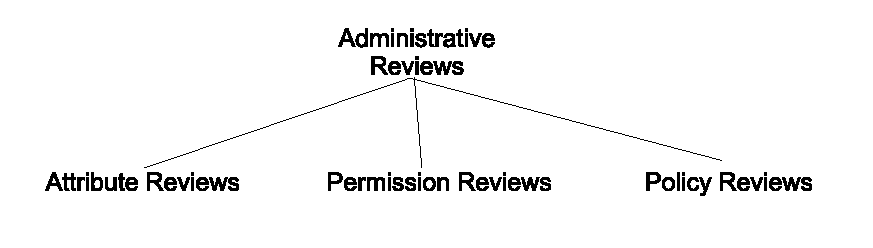
\includegraphics[width=.4\textwidth]{review-function-diagram}
		\caption{Review functions in ABAC}
		\label{fig:labac}
	\end{figure}
	

% Please add the following required packages to your document preamble:
% \usepackage{booktabs}
\begin{table}
	\centering
	\caption{Some review questions on an ABAC model} %\vspace*{3pt}
	\label{tab:review-functions-example}
	\begin{tabular}{|l|}						
		\hline					
		\multicolumn{1}{|c|}{\underline{\textit{I. Attribute Reviews }}}\\				 
		
			 1. What attributes are assigned to a user? \\
			 2. What are the values of a user attribute for a given user? \\
			 3. Which users are assigned to a given (attribute, value) pair? \\
			 4. Values of an object attribute? \\
			 5. What objects are assigned to a (attribute,value) pair ? \\
			 
		\multicolumn{1}{|c|}{\underline{\textit{II. Permission Reviews}}} \\		
		
	     	1. What permissions a user has? \\
	     	2. What permissions a user gains or looses after being assigned  \\ \hfil to a new attribute value? \\	     	 
	     	3. For a  certain permission, which attribute, values are required? \\
	     	
		\multicolumn{1}{|c|}{\underline{\textit{III. Policy Reviews}}} \\
		
			 1. Which users are allowed by a given policy? \\
			 2. Which objects are allowed by a given policy? \\
			 3. Which actions are granted by a given policy?\\
			 4. Which users (in term of (attribute, value) pair) are granted \\ \hfil what actions  on which objects (in term of (attribute, value) pair)?
		\\ \hline	
	\end{tabular}	
\end{table}


In addition to reviews on attributes, we can also pose interesting review questions on policies. While, some review questions may need to consider all  available policies in the system, some other simple reviews can be answered using a candidate policy. For simplicity, in this section, we are interested only on those simple review functions. Informally, let us assume an ABAC policy that says `users with clearance manager can approve existing loan' for user attribute `clearance' and value from the set \{manager, employee\}, object attribute `loan' and value from the set  \{existing, default\} and  and action 'approve'. Some simple review questions that we can ask using this policy include - a. who can approve existing loans ? b. which type of loan a manager can approve? c. who can approve which loans so on.

To formally define review functions, in the following section we first define a simple ABAC model - \sABAC{}. We follow the conventional approach for designing policies based on flexible policy language. In Section \ref{sec:review-function}, we define review functions using the \sABAC{} model. In Section \ref{section:np-complete}, we show that even simple policy review in \sABAC{} is NP-Complete. 

	
\newcommand{\phiu}{\phi_{u}}
\newcommand{\phio}{\phi_{o}}
\newcommand{\phia}{\phi_{a}}
\newcommand{\phip}{\phi_{p}}
\newcommand{\phix}{\phi_{x}}
\newcommand{\phiy}{\phi_{y}}
\newcommand{\userAttrExpr}{UAExpr}
\newcommand{\objectAttrExpr}{OAExpr}
\newcommand{\actionExpr}{AExpr}
\newcommand{\review}{acting\_users}
\newcommand{\simpleReview}{deep\_review}
\newcommand{\isSatisfiable}{is\_satisfiable}
\newcommand{\interpretationY}{I_y}
\newcommand{\interpretationX}{I_x}
\newcommand{\interpretation}{I}
\newcommand{\reductionAlgo}{CircuitSAT2PolicyReview}
\newcommand{\psiu}{\psi_{u}}



\subsection{\sABAC{} as a Conventional ABAC Model}
\sABAC{} model is defined for a finite set of users $U$, objects $O$ and actions $A$. Additionally, it has a set of attribute functions for users and objects. One or more user attributes form UAExpr, one of more object attributes form OAExpr and oen or more actions from AExpr.

	
\newcommand{\policyEval}{\delta}
% Please add the following required packages to your document preamble:
% \usepackage{booktabs}
\begin{table*}
	\centering
	\caption{  \sABAC{} Model} %\vspace*{3pt}
	\label{tab:labac-definition}
	\begin{tabular}{|l|}						
		\hline					
		\multicolumn{1}{|c|}{\underline{\textit{I. \sABAC{} Model } } }\\	
		
	 	- $U, O, A$: set of users, objects and actions \\
	 	- $UA,OA$: set of attribute functions for users and objects respectively.   \\ \hfill	$for_{ua \in UA}, ua: U \to 2^{range(ua)} $ and
	 	$for_{oa \in UA}, oa: O \to 2^{range(oa)} $ \\
	 	- policy: for an action, a policy $\phi_a$ is defined as shown in table \ref{tab:sabac-def}\\
	 	%-  policy: For an action a, a policy \phi_a is defined as shown table ?? \\
	 	 
	 
	 \hline	
	\end{tabular}
	
\end{table*}

%mod

	\newcommand{\UAttrVal}{\text{UAttrVal}}
\newcommand{\OAttrVal}{\text{OAttrVal}}
\newcommand{\Action}{action}
\newcommand{\E}{E}
% Please add the following required packages to your document preamble:
% \usepackage{booktabs}
\begin{table}[]
\centering
\caption{Policy Definition for \sABAC}
\label{tab:sabac-def}
\begin{tabular}{@{}l@{}}
 \hline
	$\phi ::= \phi \land \phi | \ \phi \lor \phi | \ (\phi) | \neg \phi $\\
 
	$\phi ::= \E $ \\
	Terminal Symbols:\\
	$ \E (attr: UA \cup OA, val: range(Attr))$ \\ \hfill  $\to \{true, false\}$ \\
	%$Act(\requestContext, a) \to \{true, false\}$\\
 %\bottomrule
 \\\hline
\end{tabular}
\end{table}

 
	


\subsection{Review Functions in \sABAC{}}
	

\textbf{Interpretation of Attribute Expression}\\
	Informally, an interpretation of an attribute expression  is the set of  $(attr,Value)$ pairs where $attr \in UA \cup OA$ and $Value \subseteq Range(attr)$ for which the attribute expression is evaluated to be true. Formally, we define interpretation as a function $\interpretation$ as follows.

\begin{itemize}
	\item $\interpretation(\phi) \to 2^{(attr: UA \cup OA,  Value: 2^{Range(attr)})}$ and  defined as \\
	$\interpretation(\phi) = \{(attr,Value) | (E(attr,val) \implies true ) \implies (\phi \implies true) \land val \in Value \}$
	
\end{itemize}
	
\noindent \textbf{Example of \sABAC{} Policy and its interpretation} \\
let $ \phi  \equiv \{ E(role, manager) \land \lnot E(role, dir) \land E(type, new) \}$ be a  \sABAC  policy. 	
$I_\phi = \{ (role,  \{ manager\}),$  $(type, \{ new\}), $   $(action, \{ approve\}) \}$ is satisfying interpretation for $\phi $. but $\{ (role,  \{ manager, dir\}) , (type, \{ new\}),$ \\ $(action, \{ approve\}) \}$ is not a satisfying interpretation. \\

\noindent \textbf{Review Function As a Decision Problem}
	
$\simpleReview=\{  \phi$ | exists an assignment of user and object attribute values of policy $\phi$ st. $\phi$ is evaluated true \}  \\
	
%Finally, we define review function $\reviewFunction$ as follows.$R(\phi, input:2^{\interpretation_\phi}) \to 2 ^{\interpretation_\phi}$, defined as  $R(\phi, input) = 2^{\interpretation_\phi} \setminus input$ \\	\\



 
 
% % Please add the following required packages to your document preamble:
 % \usepackage{booktabs}
 \begin{table}
 	\centering
 	\caption{Some review functions for \sABAC{}}
 	\label{tab:review-fun}
 	\begin{tabular}{|l|l|l|}
 		 \hline
 		 \textit{function Name} &  \textit{Input} &  \textit{Output}\\
 		 \hline
 		 \textit{\request} &   \{$\interpretation(\phiu), \interpretation(\phio), \interpretation(\phia)$\}&  $\delta \equiv \{true, false\}$ \\ 		 
 		 
 		 \hline
 		 \textit{UA-query} &   \{$ \interpretation(\phio), \interpretation(\phia), \delta$\}&  $\{\interpretation(\phiu)\}$ \\
		\hline
		\textit{OA-query} &   \{$ \interpretation(\phiu), \interpretation(\phia), \delta$\}&  $\{\interpretation(\phio)\}$ \\
		\hline
		\textit{Act-query} &   \{$ \interpretation(\phiu), \interpretation(\phio), \delta$\}&  $ \{ \interpretation(\phia) \}$ \\
		\hline
		\textit{UO-query} &   \{$ \interpretation(\phia), \delta$\}&  $ \{ \interpretation(\phiu),\interpretation(\phio) \}$ \\
			\hline
		\textit{deep-query} &   \{$\delta$\}&  $ \{ \interpretation(\phiu),\interpretation(\phio),  \interpretation(\phia),  \}$ \\
			\hline
 	\end{tabular}
 \end{table} 
 

  \subsection{Policy review in \sABAC{} is NP-Complete }
	
	we first informally argue that there exists a one-to-one correspondence between a boolean circuit and a policy in \sABAC{} model. Roughly, a boolean circuit is composed of n boolean variables/inputs (each denoted by $x_i$ and having a value from $\{0, 1\}$ )   and one boolean output ($y$) (in general, m outputs. But for our purpose we stick to one output). On the other hand, a \sABAC{} policy is composed of one or more functions of  $E$ which is also evaluated to be either true and false.  While boolean variable uses AND, OR and NOT gates, \sABAC{} policies uses logical $\land, \lor, \lnot$ respectively which corresponds semantically. Analogous to the output of a boolean circuit, evaluation of an \sABAC{} policy is either true or false. Thus we say a boolean circuit and a \sABAC{} policy correspond to each other. 
	
	Satisfiability of a boolean circuit asks for values of each boolean variable, $x_i$ that make the output of the circuit to be one. Similarly,  a review function (for example, in deep_review in Table \ref{table:review-fun}) may ask for possible attribute value assignments that evaluates  a access control request to be true. 
	%Each input ($x_i$) in the boolean circuit, can be thought of a evaluation function ($E$) in the UAExpr and OAExpr. \sABAC 
	
	 \subsubsection{CircuitSAT}
	 

\begin{table}[]
	\centering
	\caption{Boolean Circuit }
	\label{my-label}
	\begin{tabular}{@{}l@{}}
		\toprule
		$\psi ::= \psi \ AND \  \psi | \psi \ OR \  \psi | (\psi) | \ NOT \ \psi $ \\
		 $ \psi ::= x_i$ \\
		Terminal Symbols \\
		$x_i \in \{true, false\} $  \\		
		\bottomrule
	\end{tabular}
\end{table}

\noindent $\CircuitSAT = \{ \psi |$ there exists truth value assignments of each input $x_i$ that satisfy the boolean circuit $\psi$\} \\

	 

	
	 \textbf{NP Completeness of Policy Review} 
\begin{itemize}
	\item $\simpleReview \in NP$
		 given an instance of \simpleReview,   $\phi$  and a certificate $\interpretation$ for $\phi$. We can verify the certificate by evaluating each function $\E \in \phi$ with given attribute and values in $\interpretation$ in linear time. 
		
	\item Algorithm \ref{alg:reduction}  reduces \CircuitSAT{} to \simpleReview

	\item $\psi \in \CircuitSAT \implies \reductionAlgo(\psi) \in \simpleReview$:
		    $\psi  \in \CircuitSAT$ means there is a satisfying assignment of all $x_i \in \psi$. We replace all boolean variable, $x_i$ with evaluation function, $E_i$ resulting $\psiu$. So there must be a satisfying truth assignment of each $E_i$ satisfying $\psiu$. If we use the same (attribute, value) pairs as used in the construction of each $E_i$, we get a satisfying interpretation of attributes, $\interpretationX$ for $\psiu$.
		     %As a result, for $(\psiu \land \E(a_i, val_i), E(a_i, val_i), ( ai, \{val_i\}) )$, there is an interpretation $\interpretationX$ that satisfy $\psiu$. That means, $\reductionAlgo(\psi) \in \simpleReview$. ( because of fact that  $\reductionAlgo(\psi)$ results $(\psiu \land \E(a_i, val_i), E(a_i, val_i), ( ai, \{val_i\}) )$)
	\item $ \phi \in \simpleReview \implies \exists \psi [ \psi \in \CircuitSAT]$:	\\
		   If we replace each $\E_i$ in $\phi$ with $x_i$ resulting $\psi$, $psi$ is still satisfiable because $\phi$ is satisfiable. This implies that $\psi \in \CircuitSAT$. 
		
	\item Algorithm \ref{alg:reduction} runs in polynomial time. 
\end{itemize}
	
	
	\begin{algorithm}
	\caption{ Reduction of Circuit SAT to Policy Review Problem}
	\label{alg:reduction}
	\begin{algorithmic}[1]
		\Procedure{\reductionAlgo ($Circuit \ \psi$)}{}
		\State Replace boolean ops with logical ops.
		\For{each variable  $x$ \Pisymbol{psy}{206} $\psi$ }
		\State replace $x$ with \textbf{\E($a \in UA \cup OA, val \in range(a)$) } 
		\EndFor
		\State let $\psiu$ denote the resulting \userAttrExpr		
		\State return $\psiu$ 	
		\EndProcedure
	\end{algorithmic}
\end{algorithm}

\subsubsection{Policy Review in LaBAC is Polynomial}
%\input{labac-grammer-for-review.tex}

\section{Authorization policy representation}

\label{sec:background}
In this section, we discuss two types of authorization policies - logical-formula and enumerated policy wrt finite domain attributes based on the assumption of the finiteness of attribute values. 
\subsubsection{Finite domain ABAC}
%\textbf{Finite domain ABAC model}
	\section{Assumption of Finite Domains}
\subsection{Finite policies for Finite domain ABAC}

\textbf{Theorm 1:} \\
For L boolean variables at most $2^{2^L}$ distinct boolean expression can be defined over logical AND, OR and NOT operators. 

\textbf{Theorm 2:} \\
Let UA be the set of user attributes, OA be the set of object attributes and $A=UA \cup OA$. For an attribute $a \in A$, let $R(a)$ denote co-domain or range of the attribute. Further $OPS$ be the set of all comparison operators that compares user/object attribute with other attribute values or constant values. The maximum number of boolean variable (expression of the form (value op value) ) that can be defined comparing attribute values are $|A| \times |OP| \times \sum_{a \in A} R(a)$
	%\subsection{Enumerated \& logical-formula authorization policy}

\vspace{-.5em}
%\textbf{Logical-formula authorization policy}
\subsubsection{Logical-formula authorization policy}
Logical-formula authorization policy (\LAP{}) can be defined as a boolean expression consisting of subexpressions connected with logical operators (for example, $\land, \lor, \lnot$ and so on ) where each subexpression compares attribute values with other attribute or constant values. The language for \LAP{} usually supports a large set of logical and relational operators. A \LAP{} grants a user request for exercising certain action on an object if attributes of the requesting user and requested object evaluate the formula true. $Auth_{read} \equiv clearance(u) \succeq classification(o)$ is an example of  logical-formula authorization policy which allows a user to read an object if the user's clearance dominates classification of the object.

\LAP{}s are usually expressed in propositional logic. Examples of  \LPModels{} models  include \cite{abacAlpha,hgabac,abac-ws,abac-for-web-service}.  Flexibility of these models have been demonstrated by configuring conventional DAC\cite{dac}, MAC\cite{lbac} and RBAC \cite{rbac} policies in it. It has been shown  \cite{labac} that policy review in  \LPModels{} is equivalent to the satisfiability problem  which is NP-complete for propositional logic. 
\vspace{-1em}
%in proposition logic (or in first-order logic if LAPs are expressed in it) which makes the complexity of reviewing policies NP-complete in \LPModels{} models.


%\textbf{Enumerated authorization policy}
\subsubsection{Enumerated authorization policy}
	An enumerated authorization policy (\EAP{}) consists of a set of  tuples.  Each tuple \textit{(UAVals, OAVals)} grants privileges to a set of users  to exercise an action on a set of objects identified by the user and object attribute values \textit{UAVals} and \textit{OAVals} respectively. In an EAP, each tuple is distinct and grants privileges independently. Both  UAVals{} and OAVals{} can be atomic valued or set valued. (\textit{\manager, TS}) and (\textit{\{\manager, dir\}, \{TS,H\}}) are example of atomic and set valued tuples respectively. 
	
Usefulness of \EAP{}s have been demonstrated in the literature. For example, \textit{Policy Machine (PM)} \cite{policy-machine} and \labac{} \cite{labac} show flexibility of \EAP{}s by their ability to configure traditional models. 


%For example, in Policy Machine (PM) \cite{policy-machine}, Ferraiolo et. al define attribute based enumerated policies using one user attribute, one object attribute and a set of actions. PM also shows how to configure traditional models including DAC \cite{dac}, MAC \cite{lbac}, RBAC \cite{rbac} and Chinese wall \cite{chinese-wall}  using enumerated policies \cite{INCITS526}. On the other hand, \labac{} is another example showing usefulness of enumerated policies. A comparative analysis of enumerated authorization policy and logical-formula authorization policy is discussed in Section \ref{sec:LP-vs-EP}






%\subsection{Tripli Experssive power}


		\begin{figure*} 
		\centering
		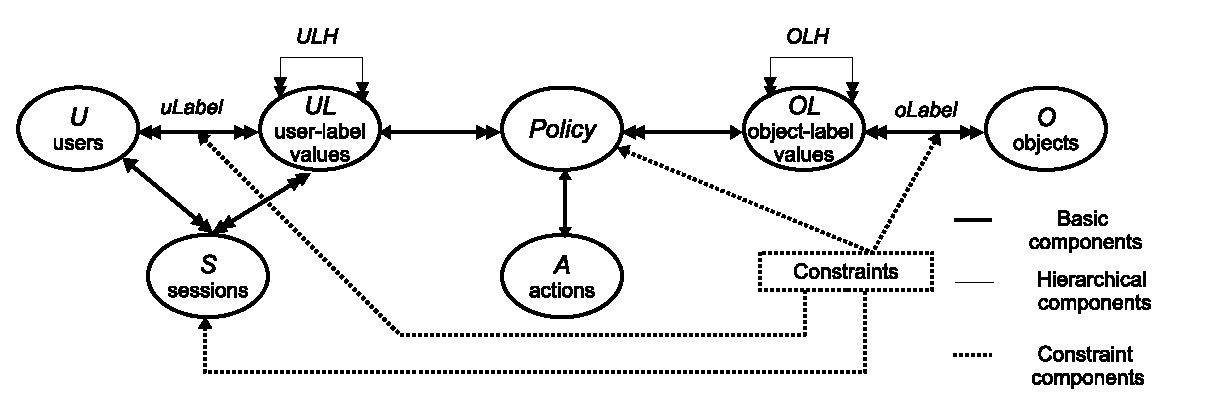
\includegraphics[width=1.1\textwidth]{ABAC16/labac-1-11}
		\caption{Components of \eapABAC{}}
		\label{fig:labac}
	\end{figure*}
	

		\begin{figure}
		\centering
		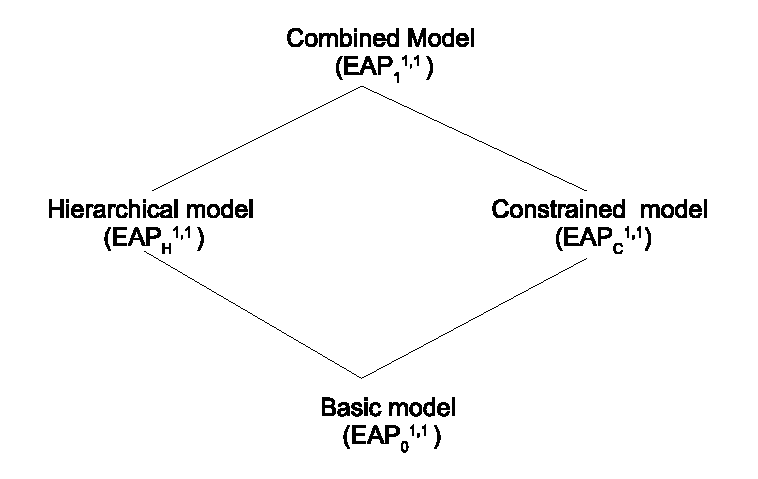
\includegraphics[width=.7\textwidth]{ABAC16/labac-family}
		\caption{Family of \eapABAC{} models}
		\label{fig:labac-family}
	\end{figure}
		
	

\section{Family of LaBAC Models}
\label{sec:model}


In this section, we describe the LaBAC model  along with formal definitions. LaBAC, short for Label Based Access Control, uses one user-label named $\uLabel$ and one object-label named $\oLabel$. We define label as a special attribute. While attributes in general have open-ended semantics, labels are associated with specific semantics. For example, attributes can be set-valued (e.g. roles or clearance) or atomic valued (e.g. age). An attribute value can be assigned by an administrator (eg. role, clearance), self-asserted (e.g. date of birth), or derived from other attributes (e.g. age can be derived from date of birth). Moreover, value of attributes can be ordered or unordered.  On the other hand, labels are set-valued, values are partially ordered and are assigned by administrators. 



For the sake of clarity and emphasis on different elements of the model, we present LaBAC as a family of models. Basic LaBAC (\clabac), presents the minimum elements to define a LaBAC model. Additionally, we add hierarchies and constraints with it in \hlabac{} and  \consLabac{} respectively.  \labacOneOneOne{} combines both the hierarchical and constrained models. The components of the LaBAC models are shown in Figure \ref{fig:labac} and the family of the models is schematically presented in Figure \ref{fig:labac-family}.
	% Please add the following required packages to your document preamble:
% \usepackage{booktabs}
\begin{table}
	\centering
	\caption{ \clabac{} Model} %\vspace*{3pt}
	\label{tab:labac-definition}
		\begin{tabular}{|l|}						
		\hline					
				\multicolumn{1}{|c|}{\underline{\textit{I. Sets and relations }}}\\			
				- $U, O$ and $S$ (set of users, objects and sessions resp.)  \\
				- $UL$, $OL$ and $A$ (finite set of user-label values, \\ \hfill object-label values and action resp.) \\
				- $uLabel$ and $oLabel$ (label functions on users and \\ \hfill objects).  $\uLabel: U \to 2^{\UL}$;   $\oLabel: O \to 2^{\OL}$ \\			
				- $\creator: S \to U$, many-to-one mapping from $S$  to $U$ \\
				- $\sessionLabels: S \to 2^{UL}$, mapping from $S$   to    $uLabel$  values. \\ \hfill
				$\sessionLabels(s) \subseteq   uLabel(\creator(s)) $ 	\\ 
				$\langle$ see Section \ref{sec:session-management} for session management functions $\rangle$\\
			%	\hfil [session management functions] \\ 
				\\ \multicolumn{1}{|c|}{\underline{\textit{II. Policy components}}} \\	
				-  $\Policy_a \subseteq \ULV \times  \OLV$,  for action $a \in A$. \\
				- $\Policy = \{ \Policy_a | a \in A  \}$ \\ \\			
				
				\multicolumn{1}{|c|}{\underline{\textit{III. Authorization function}}} \\						
				- \request(s:S,\amem:A,\objmem:O) =	 
					$\exists ul \in \sessionLabels(s) ,$ \\ \hfill $ \exists ol \in oLabel(o)$  $[ (ul,ol) \in$ $\textit{\policy}_a ]  $  		
			
 \\ \hline	
	\end{tabular}
	
\end{table}

%mod


	
\subsection{Basic LaBAC Model}
The elements represented by solid bold lines in Figure \ref{fig:labac} represent the Basic LaBAC Model (\clabac{}). In this model, a set of users, objects and actions (finite set) are represented by $U, O$ and $A$ respectively. Users are associated with a label function named $\uLabel$ and objects are associated with another label function, $\oLabel$. $\uLabel$ maps a user to one or more values from the finite set  $UL$ (represented by the double headed arrow from users to UL) and $\oLabel$ maps one object to one or more values from the finite set $OL$ (represented by the double headed arrow from objects to OL). Similarly, the double headed arrow from $UL$  to users and $OL$ to objects represent that one user-label value can be associated with more than one user and one object-label value can be associated with more than one object. 




	
Sessions are denoted by the set $S$. There is a one-to-many mapping from users to sessions. While a user  may have many $\uLabel$ values assigned to him, he can choose to activate any subset of the assigned values in a session. The relation (and function) $\creator$ and $\sessionLabels$ maintain mapping from sessions to users and sessions to $\uLabel$ values respectively.  The $\creator$ and $\sessionLabels$ functions are formally defined in Segment I of Table \ref{tab:labac-definition}. 

		
 	\begin{figure}
 		\centering
 		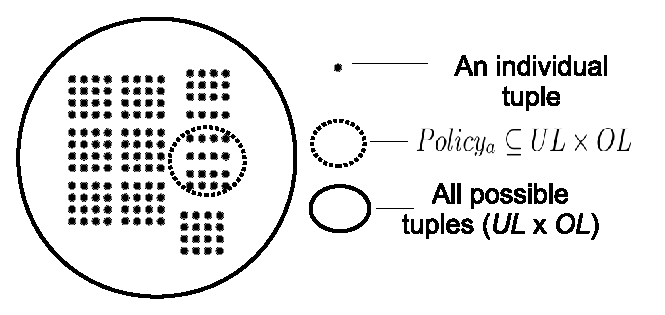
\includegraphics[width=.4\textwidth]{ABAC16/tuples-vs-policy}
 		\caption{Combining subset of tuples in a policy}
 		\label{fig:policy-vs-tuples}
 	\end{figure}	

In LaBAC, for each action, $a \in A$ we define only one policy, denoted $Policy_a$. A policy is comprised of a subset of tuples from the set of all tuples $UL\times OL$. Relationship between a policy and tuples is schematically shown  in Figure \ref{fig:policy-vs-tuples}. In defining policies, a policy may contain many tuples and a tuple $(ul,ol) \in UL\times OL$ can be used in more than one policy. Thus, a many-to-many relation exists between policies and tuples. Finally, the set \textit{\Policy} contains all individual policies for each action $a \in A$. The formal definition of \textit{\Policy{}} is shown in Segment II of Table \ref{tab:labac-definition}.

The authorization function $\request(s, a, o)$ allows  an access request by a  subject $s \in S$ to perform an action $a \in A$ on an object $o \in O$ if all following conditions are satisfied - $s$ is assigned a value $ul$;  $o$ is assigned a value $ol$ and the policy for action $a$ contains the tuple $(ul,ol)$. The formal definition of the authorization function is given in Segment III of Table \ref{tab:labac-definition}.


	
		
 	\begin{figure}
 		\centering
 		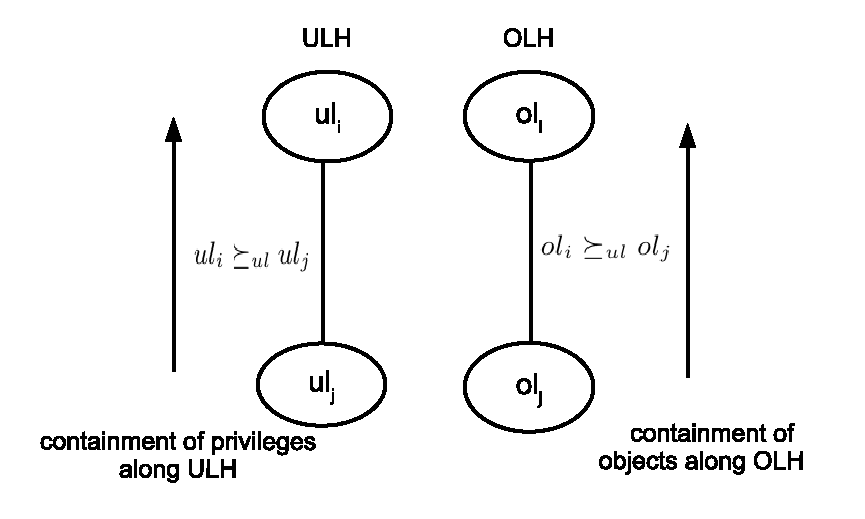
\includegraphics[width=.8\textwidth]{ABAC16/direction-of-implication}
 		\caption{ULH and OLH}
 		\label{fig:direction-of-implication}
 	\end{figure}

		
	
	
	\subsection{Hierarchical LaBAC}
	Hierarchical LaBAC model (\hlabac ) introduces user-label hierarchy ($ULH$) and object-label hierarchy ($OLH$) in addition to the components of \clabac{}. Some elements in \clabac{} are also modified in \hlabac{}. The additions and modifications in \hlabac{} from \clabac{} are shown in Table \ref{tab:labach-definition}.
	
	Hierarchy is a convenient way of ranking users and objects. LaBAC achieves ranking on users through $ULH$ and ranking on objects through $OLH$. For two user-label values, $ul_i$ and $ul_j$, when we say $ul_i$ is senior to $ul_j$ (written as $ul_i \udominate ul_j$), we mean that users assigned to $\uLabel$ value $ul_i$  can also exercise all privileges of users who are assigned to value $ul_j$. Similarly, for two object-label values, $ol_i$ and $ol_j$, when we say $ol_i$ is senior to $ol_j$ (written as $ol_i \odominate ol_j$), we mean that objects assigned to value $ol_j$ are also considered as inherited objects for value $ol_i$ for the purpose of authorization. The direction for the containment of privileges and objects along the hierarchy of $ULH$ and $OLH$ is shown in Figure \ref{fig:direction-of-implication}. For containment of objects, in Figure \ref{fig:implied-policy} objects that are assigned value `public', are also considered to be objects that are assigned  value `protected'.
	
	% For example, in Figure \ref{fig:implied-policy}, $protected \odominate public$ and   $ULH$ and $OLH$ is explained in Figure \ref{fig:direction-of-implication}.
	
	When we assign a tuple $(ul_m,ol_n)$ in a policy $\Policy_a$, additional tuples are also implied for $\Policy_a$ because of user-label and object-label value hierarchy. We identify these implied tuples with the notion of a new set $\impliedPolicy$. The implied policy  $\impliedPolicy_a$ includes all tuples of $\Policy_a$ and extra tuples that are implied by every tuples of $\Policy_a$. 
	
	%There is a one-to-one mapping between policies and implied policies.
	

	
		
		% Please add the following required packages to your document preamble:
% \usepackage{booktabs}
\begin{table}
	\centering
	 \captionsetup{justification=centering}
	 \caption{\hlabac{} Model \newline (Additions and modifications to \clabac{})}
	%\caption{  } %\vspace*{3pt}
	\label{tab:labach-definition}
		\begin{tabular}{|l|}						
		\hline								
			\multicolumn{1}{|c|}{\underline{\textit{I. Sets and relations}}} \\		
			%\multicolumn{1}{|c|}{\underline{\textit{(in addition to the basic model)}}} \\		
				  - $\ULH \subseteq \ULV \times \ULV$, partial order ($\succeq_{ul}$) on $UL$  \\
					
	              - $\OLH \subseteq \OLV \times \OLV$, partial order ($\succeq_{ol}$) on $OL$  \\ 
				  - $\sessionLabels(s) \subseteq   \{ ul' | ul \in uLabel(\creator(s)) \land ul \udominate ul' \}$		\\   \\						  				 			 	
		
			\multicolumn{1}{|c|}{\underline{\textit{II. Implied policy}}} \\
				- $\impliedPolicy_a = \{ (\ulvmem_i, \olvmem_j) |  \exists (\ulvmem_m, \olvmem_n) \in \policy_a$[  $ \ulvmem_i \udominate \ulvmem_m \land \olvmem_n \odominate \olvmem_j] \}$	\\ \hfil (explained in Figure \ref{fig:implied-policy})	\\ \\
				
				%- $\textit{\effectivePolicy}_a$ $ = \policy_a \cup \impliedPolicy_a$ \\\\
					
		 	\multicolumn{1}{|c|}{\underline{\textit{III. Authorization function}}} \\
				 
				 	- \request(s:S,\amem:A,\objmem:O) =	 
				 	$\exists ul \in \sessionLabels(s) ,$ \\ \hfill $ol \in oLabel(o)$  $[ (ul,ol) \in$ $\textit{\impliedPolicy}_a ]  $ \\					 
 \hline	
	\end{tabular}
	
\end{table}

%mod



	
 	\begin{figure}[h]
 		\centering
 		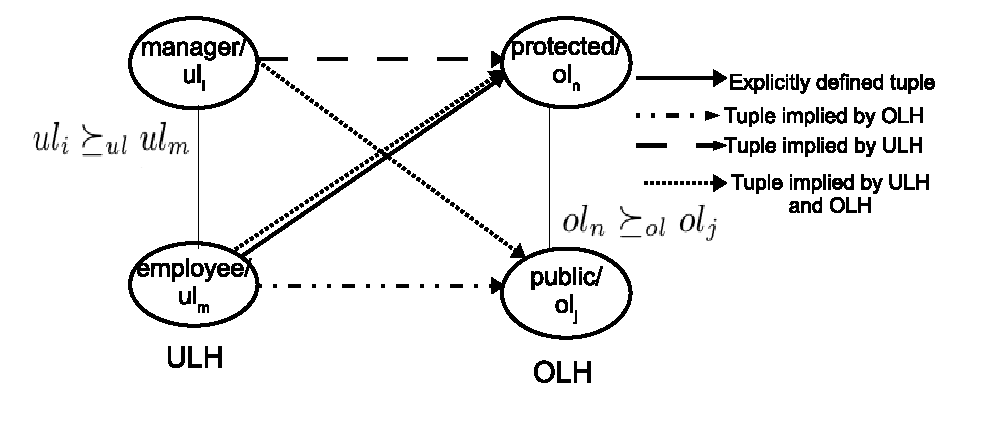
\includegraphics[width=1\textwidth]{ABAC16/implied-policy}
 		\caption{Policy and implied policy}
 		\label{fig:implied-policy}
 	\end{figure}
	
	Implied policy is  explained in Figure \ref{fig:implied-policy}.  For a policy, $\Policy_a = \{(employee, protected)\}$, corresponding implied policy is $\impliedPolicy_a=\{(manager, protected),$ \\$ (manager, public), (employee, protected), (employee, public)\}$. Figure \ref{fig:implied-policy}, further classifies tuples into tuples implied by $ULH$, or $OLH$ or both. Note that authorization function and session function are also modified in Table \ref{tab:labach-definition} to accommodate $ULH$ and $OLH$.
	


	
	
	
	%
 	\begin{figure} 
 		\centering
 		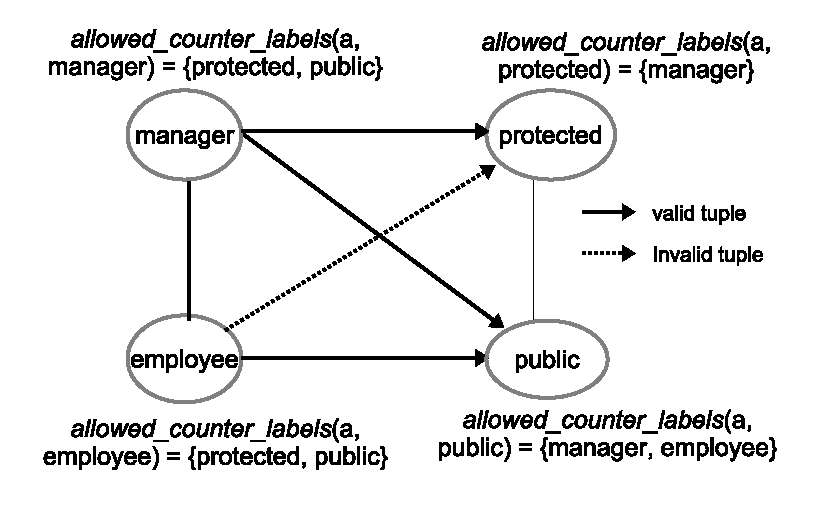
\includegraphics[width=.4\textwidth]{bound-function-explained}
 		\caption{Policy constraints explained with constraint function - \allowedLabels()}
 		\label{fig:bound-function-explained}
 	\end{figure}
	
	\subsection{Constrained LaBAC}
	A general treatment of assignment constraints in ABAC has been covered in  \cite{abcl}. similarly, role based authorization constraints have been extensively studied in \cite{rcl}.	
	In this section, we specify constraints for the LaBAC model. 
	
	We scope constraints as  means of restricting administrative or user actions. We define two types of constraints - assignment constraints and  policy constraints. Assignment constraints put constraints on user to user-label value assignments,  object to object-label value assignments and session-label value assignments. An example of user-label value assignment constraint is that a user cannot be assigned all following values $\{manager, director,$  $employee\}$.  An example of object-label value assignment constraint is that an object cannot be assigned both values - \textit{protected} and \textit{public}. An example of session-label value assignment constraint is that both \textit{manager} and \textit{director} values cannot be activated in the same session.	 Policy constraints, on the other hand,  prevent certain tuples in policies. For example, policy constraints may enforce that an \textit{employee} can never access \textit{protected} objects by restricting the tuple \textit{(employee, protected)}.  
	
	
	\begin{table}
	\centering
	\captionsetup{justification=centering}
	\caption{\consLabac{} Model  (Additions and modifications to \clabac{})} %\vspace*{3pt}
	\label{tab:constraint-definition}
%	\begin{tabular}{|l|l|}
%		\hline
		\begin{tabular}{|l|}						
			\hline					
				
				  \multicolumn{1}{|c|}{\underline{\textit{I. Components added from \clabac{}}}} \\	\\							 
					\textit{{uLabel value assignment constraint}:}\\
						  - CUL = a collection of conflicting user-label values, $\{ CUL_1, CUL_2, ... CUL_n \}$  \\ \hfil  where $CUL_i = \{ ul_1, ... ul_k\}$ \\		\\
						  
 					\textit{{oLabel value assignment constraint:}}\\
						    - COL = a collection of conflicting object-label values,$\{ COL_1, COL_2, ... COL_n \}$  \\ \hfil   where $COL_i = \{ ol_1, ... ol_k\}$ \\ \\
						    
				    \textit{{Session value assignment constraint}:}\\
					    	 - CSL = a collection of conflicting user-label values, $\{ CSL_1, CSL_2, ... CSL_n \}$   \\ \hfil  where $CSL_i = \{ ul_1, ... ul_k\}$ 	\\ \\
								  
					\textit{Policy constraint:}\\ 
						 % - $\allowedLabels(a:A, l:UL/OL) \to 2^{UL/OL}$,  \\ \hfill allowed oLabel values for   given uLabel values \\ \hfill  and vice-versa for action $a$.	\\
						 - \restrictedTuples{} $\subseteq UL \times OL$ \\
						  
			\\ \multicolumn{1}{|c|}{\underline{\textit{II. Derived components}}}	  \\ \\
						  %- $\textit{\policyBound}_a =$ \\ \hfill $ \{ (ul,ol) | \exists ul \in UL \land ol \in \allowedLabels(a,ul)\}  \cap$  \\ \hfill  $\{ (ul,ol) | \exists ol \in OL \land ul \in \allowedLabels(a,ol)\}$  \\    \\				
						  - \policyBound{} = $(UL \times OL) \setminus \restrictedTuples$ \\
			 
			
			\\ \multicolumn{1}{|c|}{\underline{\textit{III. Authorization function}}} \\	\\					
					- \request(s:S,\amem:A,\objmem:O) $\equiv$	 
					$\exists ul \in \sessionLabels(s) ,$ \\ \hfill $ \exists ol \in oLabel(o)$  $[ (ul,ol) \in$ $\textit{\policy}_a \cap \policyBound_a  ]  $  					  
			 
				 	
			 %	\multicolumn{1}{|c|}{\underline{\textit{VI. Sample Enforcement of Assignment Constraints}}} \\
			%		- $ | labels(s) \cap OneElement(CSL) | = 1$, only one  user-label \\ \hfill value can be activated in a session. 
 \\ \hline	
	\end{tabular}
	
\end{table}
	% Please add the following required packages to your document preamble:
% \usepackage{booktabs}
\begin{table}
	\centering
	\caption{ \labac{} Model} %\vspace*{3pt}
	\label{tab:labac-complete-definition}
		\begin{tabular}{|l|}						
		\hline					
				\multicolumn{1}{|c|}{\underline{\textit{I. Basic Components }}}\\			
				- $U, O$ and $S$ (set of users, objects and sessions resp.)  \\
				- $UL$, $OL$ and $A$ (finite set of user-label values, \\ \hfill object-label values and action resp.) \\
				- $uLabel$ and $oLabel$ (label functions on users and  \\ \hfill objects).  $\uLabel: U \to 2^{\UL}$;   $\oLabel: O \to 2^{\OL}$ \\				
				- $\ULH \subseteq \ULV \times \ULV$, partial order ($\succeq_{ul})$ on $UL$  \\	
				- $\OLH \subseteq \OLV \times \OLV$, partial order ($\succeq_{ol}$) on $OL$  \\ 
				- $\creator: S \to U$, mapping from $S$  to $U$ \\
				- $\sessionLabels: S \to 2^{UL}$, mapping from $S$   to $uLabel$  values.\\ \hfill	$\sessionLabels(s) \subseteq   \{ ul' | ul \in uLabel(\creator(s)) \land ul \udominate ul' \}$			\\    			  
			    %- $\allowedLabels(a:A, l:UL/OL) \to 2^{UL/OL}$,  \\ \hfill allowed oLabel values for   given uLabel values \\ \hfill  and vice-versa for action $a$.	\\\\
 			   - $\restrictedTuples \subseteq UL \times OL$ \\
 			   - \textit{CUL, COL, CSL} (conflicting set of $\uLabel, \oLabel$\\ \hfill and session-label values) \\$\langle$ see Section \ref{sec:session-management} for session management functions $\rangle$\\
			    
			   \\	\multicolumn{1}{|c|}{\underline{\textit{II. Policy components}}} \\	
			   	-  $\Policy_a \subseteq \ULV \times  \OLV$,  for action $a \in A$. \\
			   	- $\Policy = \{ \Policy_a | a \in A  \}$ \\ \\
			    
			    \multicolumn{1}{|c|}{\underline{\textit{III. Derived components}}} \\
			    - $\impliedPolicy_a = \{ (\ulvmem_i, \olvmem_j) |  \exists (\ulvmem_m, \olvmem_n) \in \policy_a$[ \\ \hfill $ \ulvmem_i \udominate \ulvmem_m \land \olvmem_n \odominate \olvmem_j] \}$	\\
			     - $\textit{\policyBound} = (UL \times OL) \setminus \restrictedTuples$ \\
			    
			    
				\\ \multicolumn{1}{|c|}{\underline{\textit{IV. Authorization function}}} \\ 						
				- \request(s:S,\amem:A,\objmem:O) =	 
					$\exists ul \in \sessionLabels(s), $ $\exists ol $ \\ \hfill   $ \in oLabel(o) [ (ul,ol) \in$ $\textit{\impliedPolicy}_a \cap  \textit{\policyBound}]  $  		
			
 \\ \hline	
	\end{tabular}
	
\end{table}

%mod


		
		 
		 
	Assignment constraints are specified by defining a set of conflicting $\uLabel$, $\oLabel$ and \textit{session} values denoted by $COL$, $CUL$ and $CSL$ respectively in Table \ref{tab:constraint-definition}.  The constraint that an object cannot be assigned both values - `protected' and `public' is specified as $COL=\{\{public, protected\}\}$ and $ |\oLabel(o) \cap OneElement(COL)| \le 1$ where function $OneElement()$ returns one element from its input set. (we use the same concept of \textit{OneElement()} from \cite{rcl}).  Similarly, other  assignment constraints can also be formulated. Note that user-label value assignment constraints can be used to configure  Static Separation of Duty, while session constraints can be used to enforce some aspects of  Dynamic Separation of Duty \cite{dsod}.


 	\begin{figure}
 		\centering
 		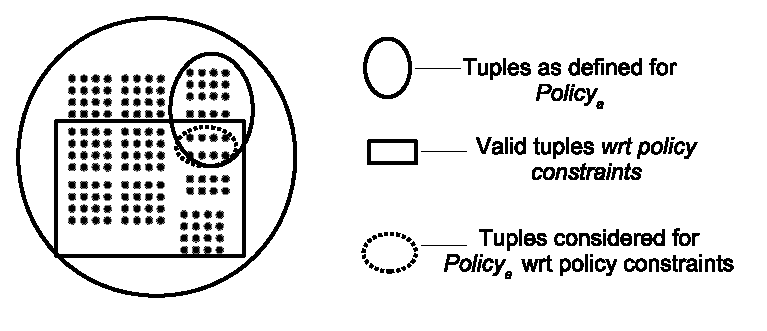
\includegraphics[width=.6\textwidth]{ABAC16/tuples-vs-valid-tuples}
 		\caption{Restricting policies with policy constraints}
 		\label{fig:tuples-vs-valid-tuples}
 	\end{figure}	


	Policy constraints are defined using the set \textit{\restrictedTuples}.  For a tuple, $(ul_r,ol_r) \in \restrictedTuples$, if it is included in a policy, $\Policy_a$, it would be ignored in the computation of authorization decision. For convenience we define a derived set \textit{\policyBound} as all possible tuples minus \textit{\restrictedTuples}. \textit{\restrictedTuples} and \textit{\policyBound} are shown in Table \ref{tab:constraint-definition}. Policy constraint is explained schematically in Figure \ref{fig:tuples-vs-valid-tuples}.
	
	In LaBAC, we include constraint policies beyond authorization policies. While, authorization policies establish relationship only between user-label and object-label values (along with actions), constraint policies go beyond. For example, constraint policies may consider relationship between \textit{UL and OL} (policy constraints), $UL$ and $UL$ (\textit{\uLabel/session} value assignment constraints), $OL$ and $OL$ (\textit{\oLabel} value assignment constraints), \textit{S and UL} (cardinality constraints on session value assignments) and so on.  As a result, constraint policies in LaBAC include logical formulas as well as enumerated tuples.
	
	
	
	
	\subsection{The Combined Model (\labacOneOneOne{})}
	
	The combined model, \labacOneOneOne{} (shown in Table \ref{tab:labac-complete-definition}), combines elements from both \hlabac{} and \consLabac{} models.  Segment I of Table \ref{tab:labac-complete-definition} presents all basic sets and relations. Policy components and derived components are shown in Segment II and  III respectively. Finally, authorization decision function is laid out in Segment IV.
	
	


%\subsection{Functional Specification}
\label{sec:session-management}
\begin{table*}
\centering
\caption{User-level session functions in \clabac{}}
\label{tab:session-management}
\begin{tabular}{|l|l|l|}
	\hline
\textbf{Fuction}                                                              & \textbf{Condition} & \textbf{Updates} \\ \hline

%\begin{tabular}[c]{@{}l@{}}\createSession\\ (u:U, s:S, values)\end{tabular} & \begin{tabular}[c]{@{}l@{}} $u \in U \land s \not \in S \land values \subseteq \uLabel(u) \setminus \{\createReq, \removeReq\}\  $ \\ $\createReq \in \uLabel(u) \land $ \\ $\exists\Policy_{\createSession} \equiv \{(\createReq, \sessionOL) \}\in \Policy$ \\ \end{tabular} &  \begin{tabular}[c]{@{}l@{}}$S' = S \cup \{s\}$ \\ $\creator(s) = u \land \sessionLabels(s)=value $ \end{tabular} \\\hline
%\multicolumn{3}{c}{\textbf{\textit{User level functions}}}\\ \hline

\begin{tabular}[c]{@{}l@{}}$\createSession$\\ $(u:U, s:S, values:2^{UL}$)\end{tabular} & \begin{tabular}[c]{@{}l@{}} $u \in U \land s \not \in S \land values \subseteq \uLabel(u)$  \end{tabular} &  \begin{tabular}[c]{@{}l@{}}$S' = S \cup \{s\}$,  $\creator(s) = u ,$ \\ $ \sessionLabels(s)=value $ \end{tabular} \\\hline


\begin{tabular}[c]{@{}l@{}}$\deleteSession$\\ $(u:U, s:S)$\end{tabular}   & \begin{tabular}[c]{@{}l@{}} $u \in U \land s  \in S \land creator(s)=u  $ \end{tabular}                   & \begin{tabular}[c]{@{}l@{}}$S' = S \setminus \{s\}$ \end{tabular}                             \\\hline


\begin{tabular}[c]{@{}l@{}}$\assignValues$\\ $(u:U,s:S, values:2^{UL}$)\end{tabular} &  \begin{tabular}[c]{@{}l@{}} $u \in U \land s  \in S \land creator(s)=u \land  values \subseteq \uLabel(u)$ \end{tabular} &   \begin{tabular}[c]{@{}l@{}} $\sessionLabels(s)= \sessionLabels(s) \cup values $ \end{tabular}                \\ \hline


\begin{tabular}[c]{@{}l@{}}$\removeValues$\\ $(u:U,s:S, values:2^{UL}$)\end{tabular} &  \begin{tabular}[c]{@{}l@{}} $u \in U \land s  \in S \land creator(s)=u \land   values \subseteq \uLabel(u)$ \end{tabular} &   \begin{tabular}[c]{@{}l@{}} $\sessionLabels(s)= \sessionLabels(s) \setminus values $ \end{tabular}                \\ \hline

%\begin{tabular}[c]{@{}l@{}}$\createObject$\\ $(s:S, o:O, values:2^{OL}$)\end{tabular} &  \begin{tabular}[c]{@{}l@{}} $s \in S \land o \not \in O \land $ \\$ f_{\createObject}(s,o, values) $ \end{tabular} &   \begin{tabular}[c]{@{}l@{}} $O' = O \cup \{o\}, \oLabel(o) = values$ \end{tabular}                \\ \hline

%\begin{tabular}[c]{@{}l@{}}$\assignLabels$\\ $(s:S, o:O, values:2^{OL}$)\end{tabular} &  \begin{tabular}[c]{@{}l@{}} $s \in S \land o  \in O \land $ \\$ f_{\assignLabels}(s,o, values) $ \end{tabular} &   \begin{tabular}[c]{@{}l@{}} $ \oLabel(o) = \oLabel(o) \cup values  $ \end{tabular}                \\ \hline

%\begin{tabular}[c]{@{}l@{}}$\removeLabels$\\ $(s:S, o:O, values:2^{OL}$)\end{tabular} &  \begin{tabular}[c]{@{}l@{}} $s \in S \land o  \in O \land $ \\$ f_{\removeLabels}(s,o, values) $ \end{tabular} &   \begin{tabular}[c]{@{}l@{}} $ \oLabel(o) = \oLabel(o) \setminus values  $ \end{tabular}                \\ \hline


%\begin{tabular}[c]{@{}l@{}}\removeValues\\ (u:U,s:S, values:2)\end{tabular} &  \begin{tabular}[c]{@{}l@{}} $u \in U \land s  \in S \land $  $\creator(s) = u \land $ $ \removeReq \in \uLabel(u) $ \\ \end{tabular} &   \begin{tabular}[c]{@{}l@{}} $\sessionLabels(s)= \sessionLabels(s) \setminus values $ \end{tabular}                \\ \hline
                 
\end{tabular}
\end{table*}



\eapABAC{} allows users to create or destroy sessions, and assign/remove values from an existing session. Table \ref{tab:session-management} presents user-level \textit{\sessionLabels{}} functions for managing sessions in \clabac{}. Each function is presented with formal parameters (given in the first column), necessary preconditions (in the second column) and resulting updates (in the third column).  The function $\createSession()$ creates a new session with given values, $\deleteSession()$ deletes an existing session, $\assignValues()$ assigns values in an existing session, and $\removeValues()$ removes values from an existing session. 

%First column in the table shows function names along with formal parameters, second column defines precondition which must be satisfied for the function to be executed. The third column describes updates in the LaBAC sets and relations once corresponding function is executed.

In \hlabac{}, we modify condition of the session functions from Table \ref{tab:session-management} to accommodate  that in a session created by a user, he can choose from the values he is assigned to or junior values. The modified conditions are given in Table \ref{tab:session-in-hlabac}. We specify an additional condition with each session function  in \consLabac{} and \labacOneOneOne{}.  For example, with $\createSession()$,  we specify a boolean function $f_{\createSession}()$ as additional precondition which must also be true. The definition of these boolean functions are  open-ended to be able to configure any session constraints. The difference between session functions in \consLabac{} and \labacOneOneOne{} is that the former does not consider hierarchy on user-label values whereas the later does. Table \ref{tab:session-in-consLabac} and \ref{tab:session-in-labacOne} show session functions in \consLabac{} and \labacOneOneOne{} respectively. Table \ref{tab:example-f-create-session} presents some examples of constraints specified with $f_{\createSession}()$ function.  \textit{Example 1} uses an enumerated policy, $\Policy_{\createSession}$. It specifies that in order to create a session and assign values to the session, a user must be assigned to value $\createReq$. \textit{Example 2} enforces the constraint that no more than one conflicting $\uLabel$ values can be activated in a session. \textit{Example 3} imposes that a user cannot have more than some bounded number of sessions.

Note that creation and deletion of objects, updating object-label values by sessions are outside the scope of \eapABAC{} operational models presented here. One reason behind is that, \eapABAC{} only focuses on attributes. It can be extended to include object creation and modification along the line of $ABAC_{\alpha}$ \cite{abacAlpha}. See Table \ref{tab:lbac-in-labac} for example.

\begin{table} 
\centering
 \captionsetup{justification=centering}
\caption{Session functions in \hlabac{} \newline (condition of session functions modified from Table \ref{tab:session-management} ) }
\label{tab:session-in-hlabac}
\begin{tabular}{|l|l|} \hline
\textbf{Function} & \textbf{Modified condition} \\ \hline
  $\createSession{}$      & \begin{tabular}[c]{@{}l@{}}  $u \in U \land s \not \in S \land values \subseteq$ \\ \hfill$  \{ ul' | \exists ul \udominate ul' [ ul \in \uLabel(u)] \}$ \end{tabular}             \\ \hline
	$\deleteSession{} $        & $u \in U \land s  \in S \land creator(s)=u  $                     \\ \hline
     $\assignValues{}$    &     \begin{tabular}[c]{@{}l@{}}  $u \in U \land s  \in S \land creator(s)=u \land values $ \\ \hfill$  \subseteq \{ ul' | \exists ul \udominate ul' [ ul \in \uLabel(u)] \}$ \end{tabular}                \\ \hline
 $\removeValues{}$    &     \begin{tabular}[c]{@{}l@{}}  $u \in U \land s  \in S \land creator(s)=u  \land values $ \\ \hfill$  \subseteq \{ ul' | \exists ul \in  \uLabel(u) \land ul \udominate ul' \}$ \end{tabular}                 \\ \hline
\end{tabular}
\end{table}



\begin{table}[]
\centering
 \captionsetup{justification=centering}
\caption{Session functions in  \consLabac{} (condition added with session functions from Table \ref{tab:session-management})}
\label{tab:session-in-consLabac}
\begin{tabular}{|l|l|} \hline
\textbf{Session function} & \textbf{Additional condition} \\ \hline
   $\createSession{}$      & $\land f_{\createSession}(u,s,values)$               \\ \hline
	$\deleteSession{} $        & $\land f_{\deleteSession}(u,s)$                     \\ \hline
     $\assignValues{}$    &      $\land f_{\assignValues}(u,s,values)$                \\ \hline
 $\removeValues{}$    &      $\land f_{\removeValues}(u,s,values)$                \\ \hline
\end{tabular}
\end{table}

\begin{table}[]
\centering
 \captionsetup{justification=centering}
\caption{Session functions in  \labacOneOneOne{} (condition added with session functions from Table \ref{tab:session-in-hlabac})}
\label{tab:session-in-labacOne}
\begin{tabular}{|l|l|} \hline
\textbf{Session function} & \textbf{Additional condition} \\ \hline
   $\createSession{}$      & $\land f_{\createSession}(u,s,values)$               \\ \hline
	$\deleteSession{} $        & $\land f_{\deleteSession}(u,s)$                     \\ \hline
     $\assignValues{}$    &      $\land f_{\assignValues}(u,s,values)$                \\ \hline
 $\removeValues{}$    &      $\land f_{\removeValues}(u,s,values)$                \\ \hline
\end{tabular}
\end{table}



\begin{table}
	\centering
 \caption{Examples of $f_{\createSession}(u, s, values)$}
 \label{tab:example-f-create-session}
	\begin{tabular}{|l|}
		\hline	                                                                                           	
		%\multicolumn{1}{|c|}{\underline{\textit{Examples in \consLabac{}/\labacOneOneOne{}:}}}\\                	
		\multicolumn{1}{|l|}{{\textit{Example 1. using LaBAC policy:}}}\\
		
		$\exists \createReq \in \uLabel(u) \land$ \\$ \exists \Policy_{\createSession} \equiv \{(\createReq, \sessionOL) \}\in \Policy$ \\
		
		\\ \multicolumn{1}{|l|}{{\textit{Example 2. using \labacOneOneOne{} session constraint CSL:}}}\\
		 $|values \cap OneElement(CSL)| <= 1$ \\
		 
		 \\\multicolumn{1}{|l|}{{\textit{Example 3. using cardinality  constraint on sessions:}}}\\
		 $|\{s | \creator(s)=u\}| <= 10$ \\
		 \hline
		\end{tabular}  

\end{table}



	 \begin{table}
\centering
\caption{Authorization policy space in \labacOneOneOne{}}
\label{tab:policy-enumeration}
\begin{tabular}{|l|l|}
\hline
\textbf{Item}                                           & \textbf{Size}               \\ \hline
Authorization policies                   & $ |A|$                       \\ \hline
Ways to define an Auth. policy       & $2^ {|UL| \times |OL|}$             \\ \hline
Ways to define all Auth. policies & $  |A| \times 2^{|UL| \times |OL|}$ \\ \hline
\end{tabular}
\end{table}
\subsection{Quantifying \labacOneOneOne{} authorization policies}
In \eapABAC{}, we define one authorization policy per action.  A policy can take any subset of all possible tuples. Thus, different number of ways to define a policy  is the size of the power set of all possible tuple as shown in Figure \ref{fig:policy-vs-tuples}.  Table \ref{tab:policy-enumeration} shows possible number of enumerated authorization policies in \labac{}.






	
	
%\section{Equivalence of LaBAC and \newline 2-sorted-RBAC}
\label{sec:equivalence}
\twoSortedRBAC{} \cite{two-sorted-rbac} is an interesting extension of Role Based Access Control which breaks the duality of roles (users and permissions perspectives) into proper roles ($\properRole$) as group of users and demarcation ($\demarcation$) as group of permissions. User inheritance is maintained with proper role hierarchy ($\properRoleHierarchy$) and permission inheritance is maintained with demarcation hierarchy ($\demarcationHierarchy$). The connection between proper roles and demarcation is maintained by the grant relation ($G$) which enumerates (proper role, demarcation) pairs. For example, for proper roles and demarcations given in Figure \ref{fig:two-sorted-rbac-example}, G includes following tuples - \{(manager, red), (employee, amber)\}. Note that \twoSortedRBAC{} \cite{two-sorted-rbac} also includes negative roles and demarcations which we do not consider here.



\twoSortedRBAC{} is compelling in many ways. It introduces a higher administrative level (through grant relation) for access management. User-role assignment ($UR^+ \subseteq U \times \properRole$) and demarcation-permission assignment ($PD^+ \subseteq P \times \demarcation$), along with administration of grant relation can be carried out more independently and distributively. Moreover, the authors shows that, \twoSortedRBAC{} enables many-to-many administrative mutations which leads to organizational scalability.  In many-to-many mutation, by granting a (proper role, demarcation) pair, all users in the proper role get all  permissions in the demarcation which, as the authors shows cannot be achieved by standard RBAC \cite{nist-rbac}.


  \begin{figure}
 	\centering
 	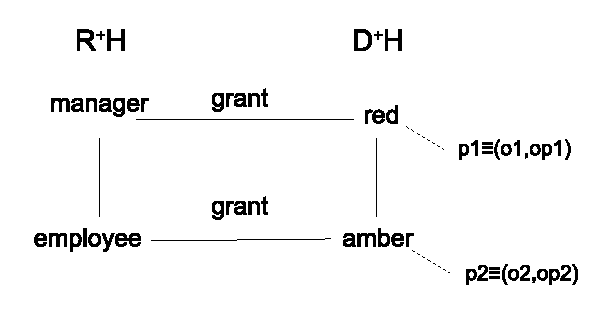
\includegraphics[width=.7\textwidth]{ABAC16/two-sorted-rbac-example}
 	\caption{An example of Two-sorted-RBAC}
 	\label{fig:two-sorted-rbac-example}
 \end{figure} 

 

The benefits of \twoSortedRBAC{} can also be realized through LaBAC. For example, user to $\uLabel{}$ value assignments, object to \oLabel{} value assignments and authorization policies are analogous to $\properRoleHierarchy$, $\demarcationHierarchy$ and grant relation in \twoSortedRBAC{} and  can also be carried out independently. On the other hand, many-to-many administrative mutation can also be achieved. For example, the LaBAC policy, $\Policy_{op1}\equiv \{(manager, (red,op1))\}$ in Figure \ref{fig:two-sorted-rbac-to-labac-example},  enables every   $manager$ to perform operation $op1$ on every object labeled with  $(red,op1)$. 

 \begin{figure}
 	\centering
 	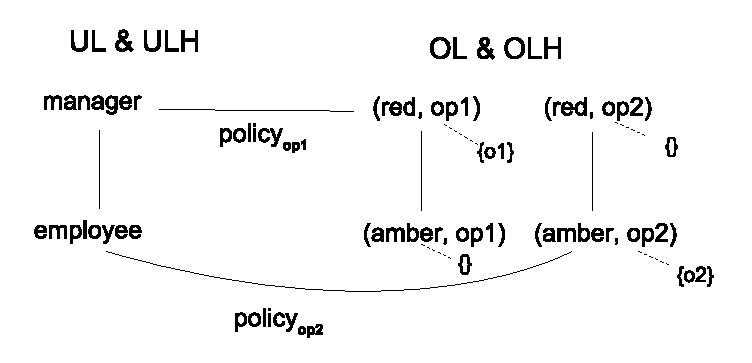
\includegraphics[width=.7\textwidth]{ABAC16/two-sorted-rbac-to-labac-example}
 	\caption{An example of \twoSortedRBAC{} configured in \eapABAC{}}
 	\label{fig:two-sorted-rbac-to-labac-example}
 \end{figure}
 


 \begin{table}
	\centering
	\caption{ \twoSortedRBAC{} in \hlabac} %\vspace*{3pt}
	\label{tab:two-sorted-rbac-in-labac-table}
	\begin{tabular}{|l|}						
		\hline					
		\multicolumn{1}{|c|}{\underline{\textit{I. \twoSortedRBAC{} components }}}\\	\\			 
		 -  $S, OBS, OPS$, $\roles, \RH$, $\demarcation, \DeH$,   (users, objects,   operations, proper roles, \\ \hfill role hierarchy, demarcation  and demarcation hierarchy respectively). \\
		 -  $PRMS = {(OBS \times OPS)}$, the set of permissions  \\		 
		 -  $\SR \subseteq S \times \roles$  \\
		 -  $\PD \subseteq PRMS \times \demarcation$ \\	 
		 - $G \subseteq \roles \times \demarcation$\\
		\\ \multicolumn{1}{|c|}{\underline{\textit{II. Construction in \hlabac{}}}} \\ \\
		 	-  $U = S, O = OBS, A = OPS $ \\ 
		 	- $UL=\roles, ULH=\RH$\\		  
		 	- $ OL = \demarcation \times OPS$\\
		 	- $OLH= \{ ((d_i, op_i), (d_j, op_j)) | d_i  \succeq d_j \land op_i = op_j\}$\\
		 	-  $\uLabel(u) = \{ r | (s,r) \in \SR \}$ \\		 	
		 	-  $ \oLabel(o) = \{ (d,op) | ((o,op),d) \in PD \}$\\		 	 	
		 	-  $\policy_{op_i} = \{ (r_i, (d_j,op_j) ) |  (r_i,d_i) \in G \land$ $((o,op_i),d_i)  \in \PD \} $ \\
		 \hline	
	\end{tabular}	

	
\end{table}

 
 In fact, LaBAC is similar to \twoSortedRBAC{} in spirit. While \twoSortedRBAC{} is more role oriented, LaBAC is attribute oriented. In the following of this section, we show equivalence of LaBAC and \twoSortedRBAC{} with respect to their theoretical  expressive power. In order to establish the equivalence, we show that any instance of \twoSortedRBAC{} can be expressed in LaBAC and vice-versa.

 
 
Figure  \ref{fig:two-sorted-rbac-to-labac-example} is an example showing configuration of a \twoSortedRBAC{} instance (given in Figure \ref{fig:two-sorted-rbac-example}) in LaBAC. In Figure  \ref{fig:two-sorted-rbac-to-labac-example}, user-label values and its hierarchy directly corresponds to roles and role hierarchy in Figure \ref{fig:two-sorted-rbac-example}. On the other hand, object-label values correspond to Cartesian product of $\demarcation$ and $OPS$.   An object-label value $(d_i, op)$ dominates another object-label value $(d_j, op)$, if demarcation $d_i$ dominates demarcation $d_j$. For example, for demarcations \{$red$, $amber$\} and operations $\{op1,op2\}$ (of Figure \ref{fig:two-sorted-rbac-example}), four object-label values have been defined where $(red,op1)$ dominates $(amber,op1)$ because $red$ dominates $amber$.  For an object-label value $(d,op)$, we assign $(d,op)$ to the object $o$ to if $(o,op)$ is a permission in demarcation $d$. For example, object $o1$ is assigned the value $(red,op1)$ because $(o1,op1)$ is  a permission in demarcation $red$.  On the other hand, user-label values assigned to a user corresponds to his assigned proper roles. Finally, having assigned object-label and user-label values, for each grant relation $(r,d) \in G$,  we specify authorization policy $Policy_{op} \equiv \{(r,(d,op))\}$ so that object labeled with $(d,op)$ are accessed by users with role $r$ for operation $op$. For example, for the grant relation $(manager,red)$ in Figure \ref{fig:two-sorted-rbac-example}, we create a policy $Policy_{op1} \equiv \{(manager, (red,op1))\}$. We do not create  policy $Policy_{op2} \equiv \{(manager, (red,op2))\}$ because there is no permission defined with operation $op2$ in demarcation $red$. Table \ref{tab:two-sorted-rbac-in-labac-table} formally  shows this configuration.
 

 
 %  \begin{figure}[!htbp]
 	\centering
 	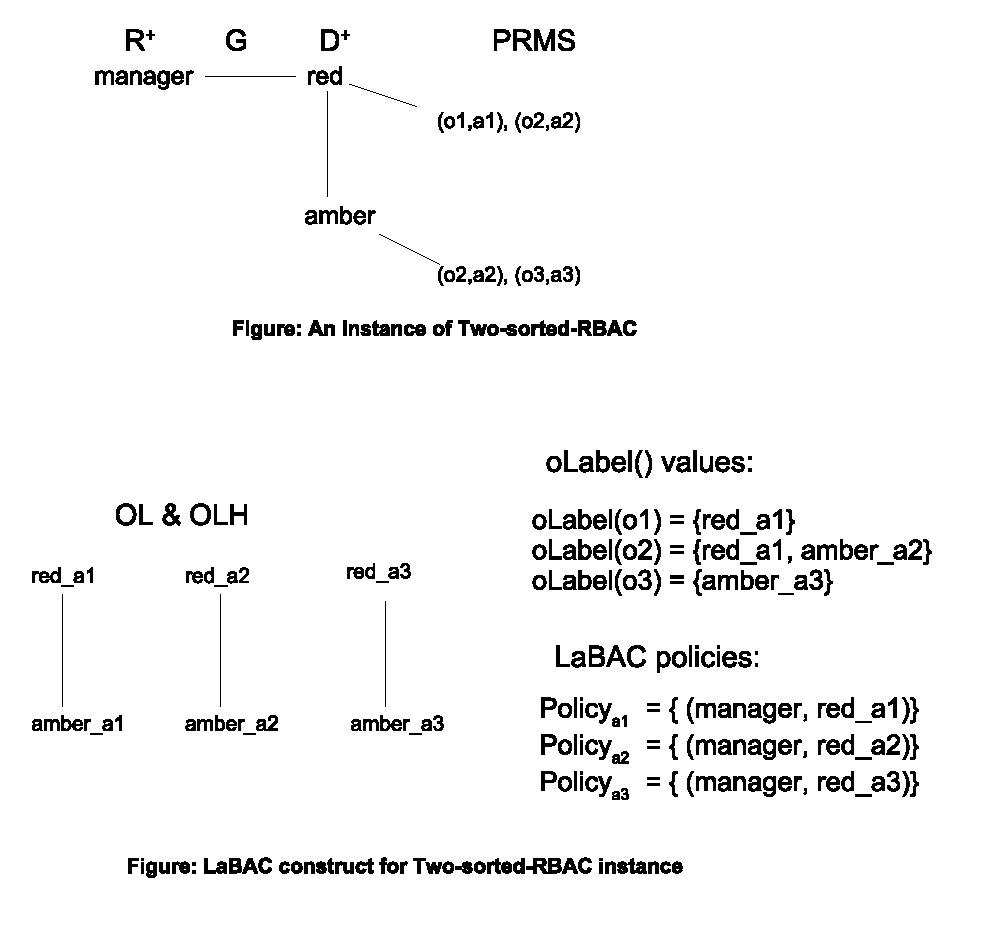
\includegraphics[width=.6\textwidth]{two-sorted-labac-example-diagram}
 	\caption{A $RBAC_1$ instance of role and perms.}
 	\label{fig:two-sorted-labac-example-diagram}
 \end{figure}
 
 \begin{table}
	\centering
	\caption{ \hlabac{} in \twoSortedRBAC{} } %\vspace*{3pt}
	\label{tab:labac-in-two-sorted-rbac-table}
	\begin{tabular}{|l|}						
		\hline					
			\multicolumn{1}{|c|}{\underline{\textit{I. \hlabac{} components}}} \\
			-  $U, O,  A$ (set of users, objects and actions resp.) \\ 
%			- $UL, OL, ULH,  OLH$ (uLabel and oLabel values, \\ \hfill uLabel and oLabel value hierarchy  resp.) \\		  
%			-  $\uLabel()$, user to user-label value assignment relation \\		 	
%			-  $\oLabel()$, object to object-label value assignment relation \\
%			-  $\policy_{a}$, LaBAC authorization policies for $a \in A$\\\\
			- $UL, OL, ULH,  OLH$ (uLabel values, oLabel values, \\ \hfill uLabel and oLabel value hierarchy  resp.) \\		  
			-  $\uLabel: U \to 2^{UL}$, $\oLabel: O \to 2^{OL}$ \\
			-  $\Policy_{a}$, authorization policy for action $a \in A$\\
		
		\\ \multicolumn{1}{|c|}{\underline{\textit{II. Construction in \twoSortedRBAC}}}\\	
		- $S=U, OBS=O, OPS=A$\\			 
		 - $\properRole = UL$, $\properRoleHierarchy = ULH$ \\ 
 		 - $\demarcation = OL$, $\demarcationHierarchy = \{\}$ \\ 
 		 - $\SR = \{ (u,r) | r \in uLabel(u)\}$\\
 		 - $\PD = \{ ((o_i, a_i), ol) | \exists (ul,ol) \in \policy_{a_i} \land$ \\ \hfill $ol' \in oLabel(o_i) \land ol \odominate ol'\}$ \\
 		 - $G = \{ (ul,ol) | (ul,ol) \in \policy_a  \}$\\
		\hline	
	\end{tabular}	

	
\end{table}

 
 
 
 Configuration of \hlabac{} in \twoSortedRBAC{} is given in Table \ref{tab:labac-in-two-sorted-rbac-table}. Segment I represents elements of LaBAC model and Segment II shows the configuration.  In the configuration, user-label values and its hierarchy are used as proper roles and proper role hierarchy. Object-label values are used as names for demarcations. For an object-label value $ol\in OL$, let $O_{ol}$ be the objects labeled with $ol$. For each policy $policy_{op} \equiv \{(ul, ol)\}$ in LaBAC, we create a grant relation $(ul,ol)$ in \twoSortedRBAC{}. Further, assign permission (o,op) in demarcation named $ol$ for $o \in O_{op}$. Note that \twoSortedRBAC{} does not distinguish between users and sessions as we do in LaBAC. For this reason, we omit LaBAC sessions while showing equivalence with \twoSortedRBAC{}.
 
 
 

  
  Here we use \hlabac{} to configure \twoSortedRBAC{} for convenience. In fact,  \clabac{} is the minimalistic model that is equivalent to \twoSortedRBAC{}. In Figure \ref{fig:expressiveness-spectrum}, we show summary of expressive power of different LaBAC models. The dashed box represents the minimalistic LaBAC model required to configure other models and solid box represents the LaBAC model that we use for our convenience. 

%We acknowledge the more formal  approach of \textit{state matching reduction} or simply \textit{reduction} \cite{tripli} for establishing equivalence between access control models. For simplicity and absence of state transition functions (administrative models) for some models discussed here, we adopt a simplified and conventional approach for the establishment of  equivalence.

The construction of Tables \ref{tab:two-sorted-rbac-in-labac-table} and \ref{tab:labac-in-two-sorted-rbac-table} and other constructions given in the rest of this paper can be cast in the formal approach of \cite{tripli}. So, these models are equivalent in the sense of state-matching reduction. 

   \begin{figure}
 	\centering
 	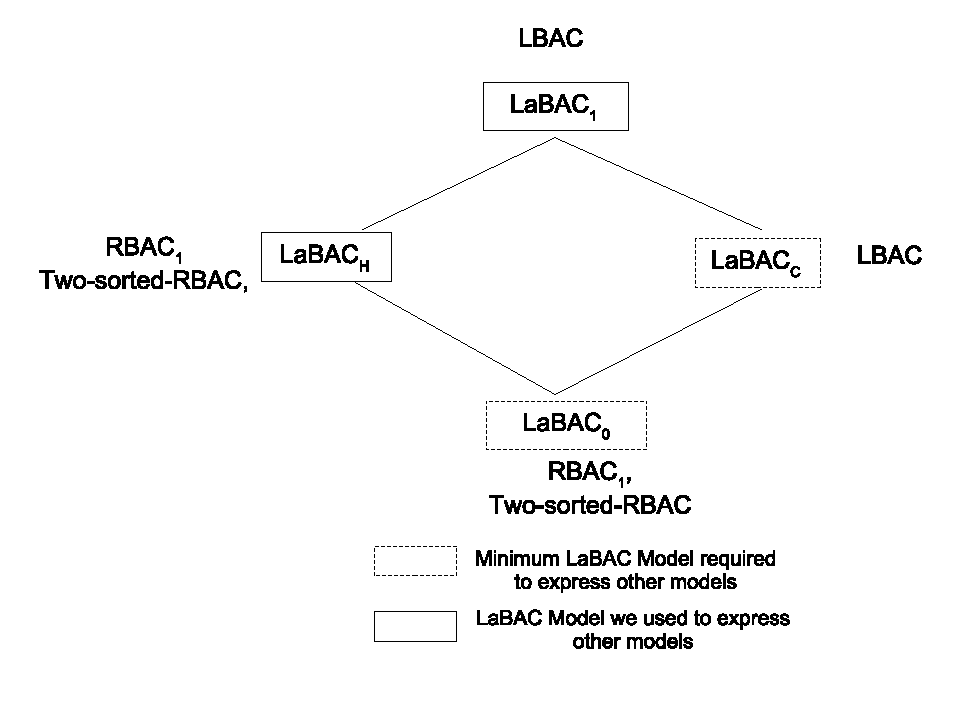
\includegraphics[width=.8\textwidth]{ABAC16/expressiveness-spectrum}
 	\caption{Expressiveness of LaBAC models}
 	\label{fig:expressiveness-spectrum}
 \end{figure}
 



%\section{LBAC and RBAC in  LaBAC}
\label{sec:configuration}
In this section, we configure LBAC \cite{lbac} and RBAC \cite{rbac}  using \labacOneOneOne{}. For each configuration, we additionally show the required number of label values and authorization policies. 

\newcommand{\latticeHead}{latticeTop} 
\newcommand{\securityClass}{SC}
\newcommand{\liberalStar}{\textit{liberal $\star$-property}}
\newcommand{\strictStar}{\textit{strict $\star$-property}}
%\subsection{LBAC in \labacOneOneOne} 




LBAC or Lattice Based Access Control is characterized by one directional information flow in a lattice of security classes. The security classes are partially ordered. One security class from these classes is assigned to each user which is known as clearance of the user. A user having a senior security class can also exercise his/her privileges using a junior  security class. For example, a top secret user can also exercise his privileges as secret user but he/she cannot use both secret and top secret clearance at the same time.  On the other hand, one security class (from the same classes of the security lattice) is assigned on objects commonly known as classification of the object. LBAC enforces one direction of information flow by two mandatory rules for reading and writing of these objects. One rule, known as \textit{simple-security property} (informally, read down rule), states that a subject (or user) can read an object if subject's clearance dominates object's classification. The other rule, known as \textit{liberal $\star$-property} (informally, write up rule),  states that a subject can write on an object if object's classification dominates subject's clearance. As a security class dominates itself it is possible to read and write  at the same level. A variation of \textit{liberal $\star$-property}, know as \textit{strict $\star$-property}, mandates that a subject can only write at his own level for the purpose of integrity requirements. A definition of LBAC is given in Segment I of Table \ref{tab:lbac-in-labac}.

\newcommand{\userLBAC}{U_{L}}
\newcommand{\objectLBAC}{O_{L}}
\newcommand{\sessionLBAC}{S_{L}}
\newcommand{\sessionUser}{sub\_creator}
\newcommand{\clearance}{clearance}
\newcommand{\classification}{classification}

\begin{table}
	\centering
	\caption{ LBAC in \labacOneOneOne{}} %\vspace*{3pt}
	\label{tab:lbac-in-labac}
	\begin{tabular}{|l|}						
		\hline					
		\multicolumn{1}{|c|}{\underline{\textit{I. LBAC components }}}\\	\\			 
		 - $\userLBAC, \objectLBAC$ and $\sessionLBAC$ (set of users, objects and sessions resp.) \\
		 -  \textit{SC}:  set of security classes in the lattice \\
		 -  \textit{SCH}: partial order on \textit{SC} (also denoted by $\succeq$ ) \\
		 - $\sessionUser: \sessionLBAC \to \userLBAC$, many-to-one mapping  from $\sessionLBAC$ to $\userLBAC$\\
		 - $\clearance: (\userLBAC \cup \sessionLBAC) \to SC$,  and  $clearance(s) \preceq \clearance(\sessionUser(s))$\\
		 - $\classification: \objectLBAC \to SC$\\		
	
		 - \textit{Simple-security property}: Subject s can read object o \\ \hfill only if \textit{clearance(s) $\succeq$ classification(o)}\\
		 - \textit{Liberal $\star$-property}: Subject s can write object o\\ \hfill only if  \textit{clearance(s) $\preceq$ classification(o)}\\
		  - \textit{Strict $\star$-property}: Subject s can write object o\\ \hfill only if  \textit{clearance(s) = classification(o)}\\
%		  - $createSession(u:\userLBAC,s:\sessionLBAC, sc:SC)$ \\ \hfill condition:$ s \not \in \sessionLBAC \land \clearance(u) \succeq sc$ \\ \hfill \hfil update: $\sessionLBAC' = \sessionLBAC \cup s$\\
		  
		  	\\	  \multicolumn{1}{|c|}{\underline{\textit{II. Construction in \labacOneOneOne{} }}} \\ \\
		  
		\\	  \multicolumn{1}{|l|}{{\textit{II(a). Construction of basic sets and relations }}} \\
		 - $U = \userLBAC, O = \objectLBAC, S = \sessionLBAC, A=\{read, write\}$\\
		 
		 - $\creator(s) = \sessionUser(s)$, for $s \in S$\\
		 -  $UL = SC,  ULH = SCH$ \\
		 - $OL = \{sc | sc \in SC \} \cup \{sc' | sc \in SC \}$\\
		 - $OLH=\{ (sc_i, sc_j) | sc_i \succeq sc_j \} \cup \{ (sc_i', sc_j') | sc_j' \succeq sc_i'\} $  [\liberalStar{}]\\
		 - $OLH=\{ (sc_i, sc_j) | sc_i \succeq sc_j \} $  [\strictStar{}]\\
		 -  $  \uLabel(u) =  clearance(u)$ \\
		 -  $  \oLabel(o) =  \{ sc, sc'\}$, where $sc=\classification(o)$	\\
		 - $ \Policy_{read} = \{ (sc_i, sc_i)| sc_i \in SC \}$ \\
		 - $ \Policy_{write} = \{ (sc_i, sc_i')| sc_i \in SC  \}$ \\
		% - Def. of  $\impliedPolicy_{op_i}$,  $\sessionLabels(s)$ for session $s \in S$ \\ \hfill and $\request(s, a, o)$  are unchanged from Table \ref{tab:labac-definition}	\\	
		 %- Session Constraints: $|\sessionLabels(s)  \cap SC| = 1$
		 
		 \\ \multicolumn{1}{|l|}{{\textit{II(b). Condition on session functions}}} \\ \\
		 - $f_{\createSession} (u, s, val) : |val|=1$\\
		 - $f_{\deleteSession}(u,s): true$\\
	     - $f_{\assignValues} (u, s, val): false$ [assuming tranquility]\\
	     - $f_{\removeValues} (u, s, val): false$ [assuming tranquility]\\
	     
	     \\ \multicolumn{1}{|c|}{\underline{\textit{III. \eapABAC{} extension for object creation}}} \\
	     - $\createObject(s,o,\{val\})$: create a new object, and    assign value $\{val\}$\\
		    \hspace{5em} condition: $s \in S \land o \not \in O \land \exists ul  \in \sessionLabels(s)  $  $ \land val \succeq ul]$ \\
		      \hspace{5em} update: $O' = O \cup \{o\}, \oLabel(o) = \{val\}$ \\
%		 - $\updateObject(s,o,\{val\})$: update $\oLabel$ value \\ \hfill of existing object\\
%		 \hfil condition: $s \in S \land o \in O \land \exists ol, \exists ul [\sessionLabels(s)=ul \land$ \\ \hfill $  \oLabel(o) = ol \land ul \udominate ol \land ul \udominate val ]$ \\
%		   \quad  update: $ \oLabel(o) = \{val\}$ 
	 \hline	
	\end{tabular}	
\end{table}



 

We present the configuration of LBAC in  \labacOneOneOne{}. Minimalistically, we need \consLabac{}  to configure some constraints of LBAC, for example, at most one security class can be activated by a subject (i.e. session in case of \eapABAC{} ) at a time. We use \labacOneOneOne{} for convenience.  

 The configuration of LBAC in \labacOneOneOne{} is given in Segment II of Table \ref{tab:lbac-in-labac}.  The security classes and its hierarchy are directly used as user label values and its hierarchy. For object-label values and its hierarchy we consider both the original lattice and the inverted lattice. The clearance of a user in LBAC  is assigned as $\uLabel$ values of the user in \eapABAC{} . On the other hand, if an object has a classification of $sc \in SC$ in LBAC,  we assign the object $\oLabel$ values of \{\textit{sc,sc'}\}, where $sc'$ correspond to $sc$ in the inverted lattice.  The \textit{simple-security} property is configured as a \eapABAC{}  policy  $\Policy_{read} \equiv \{(sc_i, sc_i)\}$ so that users having user-label value $sc_i$ can read objects having object-label value $sc_i$ or its junior.  Similarly, the $\star$-\textit{property} is configured with $\Policy_{write} \equiv \{(sc_i, sc_i')\}$ where $sc_i$ is the user-label value from the original lattice and $sc_i'$ is the object-label value from the inverted lattice and  $sc_i$  correspond to $sc_i'$. For the \liberalStar, we consider the hierarchy of the inverted lattice where as we do not consider them for the \strictStar.  An example of LBAC configured in \labacOneOneOne{} is given in Figure \ref{fig:lbac-labac-example}.

 \begin{figure}
 	\centering
 	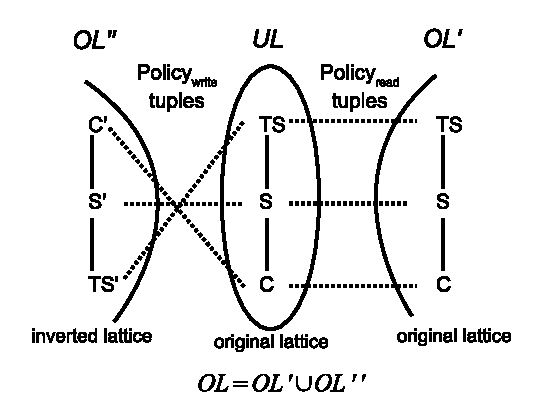
\includegraphics[width=.5\textwidth]{ABAC16/lbac-labac-example}
 	\caption{LBAC example configured in \eapABAC{}}
 	\label{fig:lbac-labac-example}
 \end{figure}
\begin{table} 
	\centering
 \caption{Quantifying LaBAC for simulating LBAC}
 \label{tab:lbac-labac-quantification}
	\begin{tabular}{|l|}
		\hline	                                                                                                           	

		$|UL| = |SC|$ and $|OL| =  2 * |SC|  $\\
		$|\Policy| = 2$  $(\Policy_{read} $ and $\Policy_{write})$\\
		%|\policy_{read}| =  1$\\
		%|\policy_{write}| =  1$\\
		\hline
		\end{tabular}  

\end{table}

Segment II(b) of Table \ref{tab:lbac-in-labac} specifies conditions for the session management functions in \eapABAC{} . In  $\createSession()$ we specify additional condition so that at most one user-label value can be activated in one session. We assume, once created clearance of subjects and classification of objects cannot be changed. This property in known \textit{tranquility} in the literature \cite{lbac}
  
Segment III is an extension of \labacOneOneOne{} for the purpose of creating objects in \eapABAC{} . Since functional specification of \labacOneOneOne{} does not include functions for creating or managing objects,  here we define a function $\createObject()$ for this purpose. We follow the \liberalStar{} as the precondition for creation of objects. 

%and $\updateObject()$ to capture creation of new objects and modification of object classification values in LBAC. The prerequisite conditions and necessary updates for execution of these functions are also presented here. 


Finally, Table \ref{tab:lbac-labac-quantification} shows required number of authorization policies, $UL$ and $OL$ values  for configuring LBAC.

%to configure LBAC in \labacOneOneOne{}.

%we quantify required number of required \labacOneOneOne{} policies for configuring LBAC which is shown in Table \ref{tab:lbac-labac-quantification}. As we can see, we need as many read and write policies as the number of security classes in the lattice.



 

 % \begin{figure*}
 	\centering
 	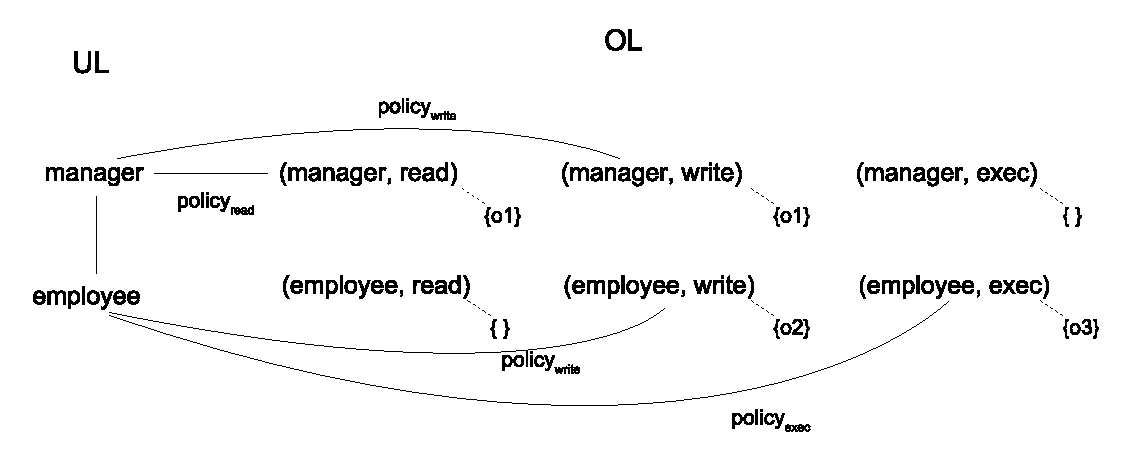
\includegraphics[width=.8\textwidth]{ABAC16/rbac-labac-configuration-explained}
 	\caption{An instance of RBAC (from Figure \ref{fig:rbac-labac-example}) configured in \eapABAC{}.}
 	\label{fig:rbac-labac-configuration-explained}
 \end{figure*}
 \newcommand{\associatedObj}{associated\_obj}

 \begin{figure}
 	\centering
 	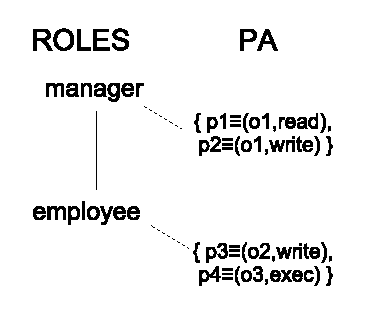
\includegraphics[width=.3\textwidth]{ABAC16/rbac-labac-example}
 	\caption{An example of roles and permission-role assignments in RBAC.}
 	\label{fig:rbac-labac-example}
 \end{figure}
 \begin{figure*}
 	\centering
 	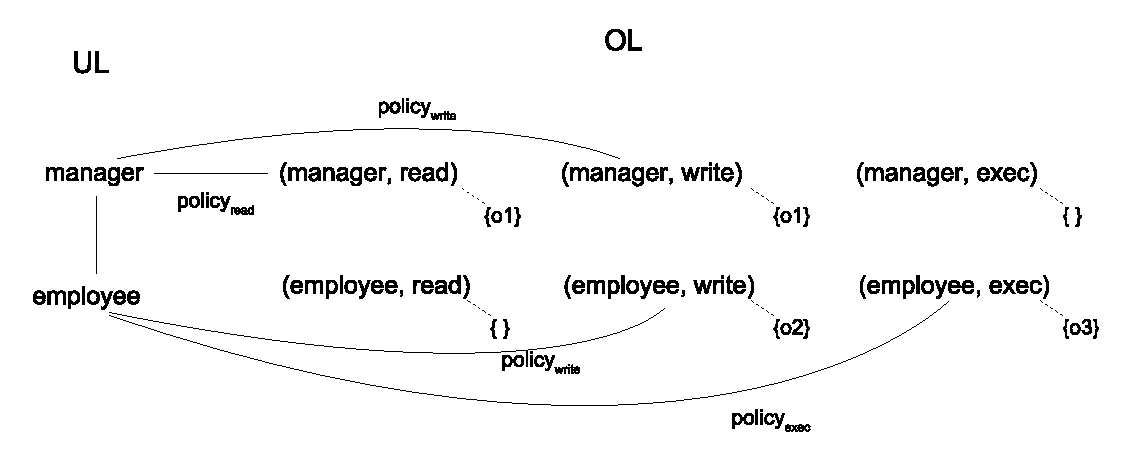
\includegraphics[width=.8\textwidth]{ABAC16/rbac-labac-configuration-explained}
 	\caption{An instance of RBAC (from Figure \ref{fig:rbac-labac-example}) configured in \eapABAC{}.}
 	\label{fig:rbac-labac-configuration-explained}
 \end{figure*}


 
%\begin{table}[]
\centering
\caption{Authorization policies in \hlabac{}  illustrating roles  in Figure \ref{fig:rbac-labac-example}}
\label{tab:rbac-labac-example-table}
\begin{tabular}{|l|l|l|l|}
	\hline
UL  & OL                                                                   & oLabel(o)                                                                          & Policy                                                                                                                                               \\
\hline
mng & \begin{tabular}[c]{@{}l@{}}\{mng\_read,\\ mng\_write\}\end{tabular}  & \begin{tabular}[c]{@{}l@{}}oLabel(o1)=\\ \{mng\_read, \\ mng\_write\}\end{tabular} & \begin{tabular}[c]{@{}l@{}} $p_{read} \equiv$ \\$\{(mng, mng\_read) \}$,\\ $p_{write} \equiv$ \\ $\{(mng, mng\_write)$,\}\end{tabular} \\ 
\hline
emp & \begin{tabular}[c]{@{}l@{}}\{emp\_write, \\ emp\_exec\}\end{tabular} & \begin{tabular}[c]{@{}l@{}}oLabel(o2)=\\ \{emp\_write, \\ emp\_exec\}\end{tabular} & \begin{tabular}[c]{@{}l@{}}$p_{read} \equiv$ \\ $\{(emp, emp\_write)\}$,\\ $p_{exec} \equiv $ \\ $\{(emp,  emp\_exec)\}$\end{tabular}       \\
\hline                                               
\end{tabular}
\end{table}



\newcommand{\sessionRoles}{session\_roles}
\begin{table}
	\centering
	\caption{ $RBAC_1$ in \hlabac} %\vspace*{3pt}
	\label{tab:rbac-in-labac-table}
	\begin{tabular}{|l|}						
		\hline					
		\multicolumn{1}{|c|}{\underline{\textit{I. $RBAC_1$ components }}}\\				 
		 -  \textit{USERS, OBS, OPS, SESSIONS, ROLES} and \textit{RH} \\ \hfill (users,  objects, operations, sessions, roles \\ \hfill and role hierarchy resp.) \\
		 -  $\textit{PRMS} = {(\textit{OBS} \times \textit{OPS})}$, the set of permissions  \\		 
		 -  $\textit{UA} \subseteq \textit{USERS} \times \textit{ROLES}$.  \\
		 - $\textit{PA} \subseteq \textit{PRMS} \times \textit{ROLES}$. \\	
		 - $session\_user: \textit{SESSIONS} \to USERS$ \\
		 %- $\sessionRoles: \textit{SESSIONS} \to 2^{\textit{ROLES}}$ ; $\sessionRoles(s) \subseteq$ \\ \hfill  $  \{r | (\exists r' \succeq r)[session\_user(s),r') \in \textit{UA}]\}$\\
		  - $\sessionRoles: \textit{SESSIONS} \to 2^{\textit{ROLES}}$ and \\ \hfill $\sessionRoles(s) \subseteq  \{r | (\exists r' \succeq r)[session\_user(s),r') \in \textit{UA}]\}$\\
		\\\multicolumn{1}{|c|}{\underline{\textit{II. Construction in \hlabac}}} \\
		 	-  $U = \textit{USERS}, O = \textit{OBS}, A = \textit{OPS}, S=\textit{SESSIONS} $ \\ 
		 	- \textit{UL=ROLES, ULH=RH}\\		  
		 	- $ OL = \textit{ROLES} \times \textit{OPS}$, $\textit{OLH}= \{ \}$\\
		 	-  $\uLabel(u) = \{ r | (u,r) \in UA \}$ \\
		 	
		 	-  $ \oLabel(o) = \{ (r,op) | ((o,op),r) \in PA \}$\\
		 	- $\creator(s) = session\_user(s)$, for $s \in S$	\\
		 	- $\sessionLabels(s) = \sessionRoles(s)$, for $s \in S$\\
		 	-  $\policy_{op_i} = \{ (r, (r',op_i) ) |  ((o,op_i),r')  \in PA \land r' = r  \} $ \\
		 	%- $\impliedPolicy_{op_i}$ and $\request()$ functions  are \\ \hfill unchanged from Table \ref{tab:labac-definition}	\\	
		 	
%		 	 \\ \multicolumn{1}{|c|}{\underline{\textit{III. Condition on session functions}}} \\
%		 	 - $\createSession(u,s,values)$: \\ \hfil $u \in U \land s \not \in S \land values \subseteq \uLabel(u)$\\
%		 	 - $\deleteSession(u,s)$: \\ \hfil $u \in U \land s \in S \land \creator(s)=u$\\
%		 	 - $\assignValues(u,s,values)$: \\ \hfil $u \in U \land s \in S \land \creator(s)=u \land values \subseteq \uLabel(u)  $ \\ 
%		 	 - $\removeValues(u,s,value)$: \\ \hfil $u \in U \land s \in S \land \creator(s)=u \land value \subseteq \uLabel(u)$ \\
		 	
		 \hline	
	\end{tabular}	

	
\end{table}

 
%\subsection{RBAC in \hlabac} 
A definition of hierarchical RBAC ($RBAC_1$) is shown in Segment I of Table \ref{tab:rbac-in-labac-table}. In RBAC, permissions are assigned to roles and users receive permissions through their enrollment to roles. Roles are partially ordered. If a role, $r_i$ is senior to role, $r_j$ (otherwise told $r_i$ dominates $r_j$), $r_i$ inherits permissions from $r_j$ and $r_j$ inherits users from $r_i$. Thus role hierarchy serves dual purpose of inheriting users and permissions. Figure \ref{fig:rbac-labac-example} presents an example showing roles, role hierarchy and permission-role assignments in $RBAC_1$. 

In Segment II of Table \ref{tab:rbac-in-labac-table}, we show  construction of $RBAC_1$ in \hlabac. Minimalistically, we need \clabac{}, but we use \hlabac{} for convenience. 



Figure  \ref{fig:rbac-labac-configuration-explained} shows an instance of RBAC (given in Figure \ref{fig:rbac-labac-example}) configured in LaBAC. In the figure, user-label values and its hierarchy directly correspond to roles and role hierarchy of Figure \ref{fig:rbac-labac-example}. On the other hand, object-label values correspond to Cartesian Product of $ROLES$ and $OPS$.   For example, for roles \{$manager, employee$\} and operations $\{read, write, exec\}$ of Figure \ref{fig:rbac-labac-example}, six different object-label values have been defined.  For an object-label value $(r,op)$, we assign it to the object $o$  if $(o,op)$ is a permission assigned to role $r$. For example, object $o1$ is assigned to label $(manager,read)$ because $(o1,read)$ is  a permission of role $manager$ (see Figure \ref{fig:rbac-labac-example}). Having assigned object-label and user-label values, for each $r \in ROLES$,  we specify authorization policy $\Policy_{op} \equiv \{(r,(r,op))\}$ so that object labeled with $(r,op)$ are accessed by users labeled with role $r$ for operation $op$. For example, for role, $manager$ in Figure \ref{fig:rbac-labac-example}, we create $\policy_{read} \equiv \{(manager, (manager,read))\}$ and $\policy_{write} \equiv \{(manager, (manager,write))\}$. We do not create  policy $\policy_{exec} \equiv \{(manager, (manager, exec))\}$ because there is no permission defined with operation $exec$ in role $manager$. Table \ref{tab:rbac-in-labac-table} formally shows the configuration of $RBAC_1$ in LaBAC. 




\begin{table} 
	\centering
 \caption{Quantifying \eapABAC{} for simulating RBAC}
 \label{tab:rbac-labac-quantification}
 
 	\begin{tabular}{|l|}
 		\hline	                                                                                                           	
 		
 	$|UL| = |ROLES|$\\ 
 	$|OL| = |ROLES| \times |OPS|$\\
 	$|\Policy| = |OPS|$\\
 		\hline
 	\end{tabular}  
\end{table}
 
 

 
 Finally, Table \ref{tab:rbac-labac-quantification} presents number of user-label values, object-label values and authorization policies required to configure $RBAC_1$.  
 


 





%\subsection{DAC in \clabac}

 
% Please add the following required packages to your document preamble:
% \usepackage{booktabs}
\begin{table*}
	\centering
	\caption{ DAC in \labacOneOneOne{} for finite users and objects} %\vspace*{3pt}
	\label{tab:dac-definition}
	\begin{tabular}{|l|}						
		\hline					
	 
		\multicolumn{1}{|c|}{\underline{\textit{I. Construction}}} \\
		- let $OID$ be finite set of object ids. \\
		-  $U, A$, be finite set of users, and actions\\
		- $O$, set of existing objects. \\
		-   $OL=OID$, $UL=\{ id(u) | u \in U \}$, for \\ \hfill $id(u)$ as the unique id of a user. \\
		- $\policy$, set of existing policies.\\
		\multicolumn{1}{|c|}{\underline{\textit{II. Administrative Actions Required for DAC}}} \\
			- let $\canAddPolicy \subseteq U \times 2^{UL} \times A \times 2^{OL}$, \\  \hfill be an administrative relation.  $(au, X, a, Z) \in \canAddPolicy$ \\  \hfill implies that  administrative user, $au$  can add/remove \\ \hfill  policy,  $policy_a \equiv (x:X,z:Z)$\\
		\multicolumn{1}{|c|}{\underline{\textit{III. create new object}}} \\
			- $create\_object(u:U, oid:OID)$ \{ \\
			\quad $o = create\_new(oid)$ \\
			\quad	$oLabel(o) = \{oid\}$\\
			\quad	$\policy = \policy \cup \{ ( id(u), read, oid), ( id(u), write, oid) )\}$ \\
			\quad   $\canAddPolicy = \canAddPolicy \cup \{(u, UL, A, \{oid \}) \}$ \\		
			\quad \} \\
			\hline
	\end{tabular}	
\end{table*}



\section{\hlabac{} in Policy Machine}
\label{sec:pm}


In this section, we show how LaBAC can be presented as a simple instance of Policy Machine (PM) \cite{policy-machine}. In order to do so, we first define Policy Machine Mini ($\pmMini{}$) - a step down version of PM sufficient enough for our purpose. We then configure \hlabac{} in $\pmMini{}$.

\subsection{$\pmMini{}$}

$\pmMini{}$ is a sufficiently reduced version of PM.  For example, while PM uses four basic relations namely Assignment, Association, Prohibition and Obligation, $\pmMini$ includes only the first two of these. Similarly, PM manages both resource operations and administrative actions but $\pmMini$ is limited to managing operation on resources only.  Additionally, \textit{Policy Class}, an important concept in PM for combining multiple policies, is not considered in $\pmMini$. 




Definition of $\pmMini{}$ is shown in Table \ref{tab:poilcy-machine-mini}. In $\pmMini{}$ users, objects, operations and processes are denoted by set $U, O, OP$ and $P$ respectively. $UA$ and $OA$ represent the finite sets of user attributes and object attributes. The definition of attributes in $\pmMini$ is different than the definition of attributes in most other models. While typically attributes are used as (attribute, value) pairs, $\pmMini$ uses attributes  as containers for users, objects and other attributes (constraints apply). For example, a user can be assigned to a user attribute $ua_i$ which can further be assigned to another user attribute $ua_j$. Same type of assignment applies for object and object attributes. User (or user attribute) to user-attribute  assignments and object (or object attribute) to object-attribute assignments are captured by the \textit{\assignment}{} relation which must be acyclic and irreflexive. On the other hand, the \textit{\association}{} relation is like a grant relation. The meaning of $(ua,\{a\},oa) \in \textit{\association}$ is that users contained in $ua$ can perform operation $a$ on objects contained in $oa$. Containment of users and objects can be transitive which is specified by the $\assignmentPlus{}$ relation. The decision function  $\decisionFunction(p,op,o)$ allows a process, $p$ (running on behalf of a user, $u$) to perform an operation, $op$ on an object, $o$ if there exists an entry, $(ua,\{op\},oa)$ in \textit{\association}{} relation  where $ua$ transitively contains $u$ and $oa$ transitively contains $o$.

\newcommand{\processUser}{process\_user}


% Please add the following required packages to your document preamble:
% \usepackage{booktabs}
\begin{table}
	\centering
	\caption{ $\pmMini$ definition} %\vspace*{3pt}
	\label{tab:poilcy-machine-mini}
	\begin{tabular}{|l|}						
		\hline					
		\multicolumn{1}{|c|}{\underline{\textit{I. Basic sets and relations }}}\\				 
		 - $U, O, OP$ and $P$ (set of users, objects, operations \\ \hfill  and processes resp.) \\ 
		 - $UA, OA$ (set of user and object attributes) \\  
		 - $AR$ (set of access rights).   In $\pmMini$, $AR=OP$ \\
		 - $\processUser: P \to U$\\	 
		
		\\ \multicolumn{1}{|c|}{\underline{\textit{II. Assignment and association relations}}} \\
			- $\assignment \subseteq (U \times UA) \cup (UA \times UA) \cup (O \times OA)$ \\ \hfill $\cup (OA \times OA),$  an irreflexive, acyclic relation \\
	 
	
		- $\association \subseteq UA \times 2^{AR} \times OA$ \\
	 
		 \\ \multicolumn{1}{|c|}{\underline{\textit{III. Derived relations}}} \\
	 	
		 - $\assignmentPlus$, transitive closure  of $\assignment$   \\		 
	 
	 	
	 
	 	\\ \multicolumn{1}{|c|}{\underline{\textit{IV. Decision function}}} \\
	 	% - $\decisionFunction(p,a,o) = \exists(ua, ars, oa)$  $\in \associationPolicy$   \\ \hfill $[ (u,ua) \in \assignmentUAUA \land (o,oa) \in \assignmentOAOA \land a \in ars]$ 
	 	 
	 	- $\decisionFunction(p,op,o) $ =\\ \hfill $\exists oa \in OA, \exists ua \in UA, \exists u \in U $ \\ \hfill $[(ua,\{op\}, oa) \in \association \land$ \\ \hfill $ (u,ua) \in \assignmentPlus\land (o,oa) \in \assignmentPlus \land $  \\ \hfill$\processUser(p) = u]$ 	
		 	
 		\\ \hline	
	\end{tabular}	

	
\end{table}


A process in $\pmMini{}$ simply inherits all attributes of the creating user. Thus $\pmMini{}$ lacks the ability to model sessions, since there is no user control over a process's attributes.  Note that PM achieves this effect through obligation and prohibition relations \cite{INCITS526}. A complete and detailed model of Policy Machine can be found here \cite{INCITS526,policy-machine}.

  % In modeling sessions,  $\pmMini$ lacks the ability to model sessions like they are modeled (Section \ref{sec:session-management}) in LaBAC. Note that PM achieves these through Obligation and Prohibition relations \cite{INCITS526}. For curious readers, a complete and detailed model of Policy Machine can be found here \cite{INCITS526,policy-machine}.

 \subsection{\hlabac{} in $\pmMini{}$}
 \begin{table}
	\centering
	\caption{ \hlabac{} in $\pmMini{}$ } %\vspace*{3pt}
	\label{tab:labac-in-policy-machine}
	\begin{tabular}{|l|}						
		\hline					
			\multicolumn{1}{|c|}{\underline{\textit{I. \hlabac{} components}}} \\
			-  $U_L, O_L,  A, S$ (set of users, objects, actions \\ \hfill and sessions  resp.) \\ 
			- $UL, OL, ULH,  OLH$ (uLabel values, oLabel values, \\ \hfill uLabel and oLabel value hierarchy  resp.) \\		  
			-  $\uLabel: U \to 2^{UL}$, $\oLabel: O \to 2^{OL}$ \\
			-  $\Policy_{a}$, authorization policy for action $a \in A$\\
			- $\creator: S \to U$\\
		   
		\\ \multicolumn{1}{|c|}{\underline{\textit{II. Construction}}}\\	
		- $ U=U_L, O=O_L, OP=A, P = S $\\
		- $\processUser(s) = \creator(s)$, for $s \in S$\\
		- $UA = UL, OA=OL$ \\		
		- $\assignment$ = $\{(u,ul) | ul \in \uLabel(u) \} \cup$  \\ \hfil 
										$\{(ul_i, ul_j) | ul_i \udominate ul_j \} \cup$ \\ \hfil
										$\{(o,ol) | ol \in \oLabel(o) \}\cup $ \\ \hfil
										$\{(ol_i, ol_j) | ol_j \udominate ol_i \}$ \\
		- $\association= \{ (ul, a, ol) | \exists (ul,ol) \in \Policy_a$ \\ \hfill $ \land \Policy_a \in \Policy \}$ 

		\\ \hline	
	\end{tabular}	

	
\end{table}

As $\pmMini{}$ lacks the ability to manage sessions, here we present a mapping from $\pmMini{}$ to \hlabac{} without session management. In the mapping, users, objects, actions and sessions in LaBAC are directly mapped to users, objects, operations and processes in $\pmMini{}$.  User-label values and object-label values in LaBAC correspond to $UA$ and $OA$ respectively. Additionally,  user to user-label value assignments, object to object-label value assignments,  $ULH$ and $OLH$ in \hlabac{} is mapped to the \assignment{} relation. Finally, each tuple in each policy in LaBAC is contained in the \association{} relation. A mapping from  $\pmMini{}$ to \hlabac{} is given in Table \ref{tab:labac-in-policy-machine}. 

%\vfill \break 



%\section{Comparative Analysis of the ABAC Models}
	
	
	\subsection{Abstract Policy \& Policy Space}
	\newcommand{\uSubset}{U_S}
\newcommand{\oSubset}{O_S}
\newcommand{\UAExpr}{UAExpr}
\newcommand{\OAExpr}{OAExpr}
\newcommand{\uSelector}{USERs}
\newcommand{\oSelector}{OBJECTs}
\newcommand{\policySpace}{PolicySpace}

  \begin{table} 
\centering
\caption{One abstract policy represented by different \sABAC{} policies}
\label{table:sabac-def}
\begin{tabular}{@{}l@{}}
 \toprule	
	 $  E(role(u), \{manager, employee\}) \land E(type(o),\{new\} )$\\
	 $  E(role(u), \{manager\}) \land E(role(u), \{employee\}) \land E(type(o),\{new\} )$\\
	 $ \lnot E(role(u), \{\}) \land E(role(u), \{employee\}) \land E(type(o),\{new\} )$\\
 	 $ \lnot (\lnot (E(role(u), \{manager, employee\}))) \land E(type(o),\{new\} )$\\
 \bottomrule
\end{tabular}
\end{table}
 
 \textbf{Abstract Policy}
 We define abstract policy as a tuple of following forms - $(\uSubset, a, \oSubset)$ and $(\UAExpr, a, \OAExpr)$, where $\uSubset \subseteq U$ and $\oSubset \subseteq O$, $\uSelector(\UAExpr) \subseteq U$ and $\oSelector(\OAExpr) \subseteq O$, for function $\uSelector()$ and $\oSelector()$ which specifies set of users and objects for given user attribute expression and object attribute expression. Examples of abstract policy are $(\{ Alice, Bob\}, read, \{ o1, o2\} )$ or $( E(role(u), \{manager \}), read, E(\{ type(o), \{sensitive\} ) ) $
 
 We say two abstract policies $\rho_i \equiv (\UAExpr_i, a, \OAExpr_i)$ and   $\rho_j \equiv (\UAExpr_j, a, \OAExpr_j)$ are different ($\rho_i \neq \rho_j$) iff either or both of following conditions are true.
 \begin{enumerate}
 	\item $\uSelector(\UAExpr_i) \neq  \uSelector(\UAExpr_j) \lor U_i \neq U_j$  
 	\item $\oSelector(\OAExpr_i) \neq  \oSelector(\OAExpr_j) \lor O_i \neq O_j$
 \end{enumerate}

Informally, \policySpace{} of an model is the set of all distinct abstract policies of the model. For simplicity, here we are only interested about the size of the \policySpace{}.

	\begin{figure} 
		\centering
		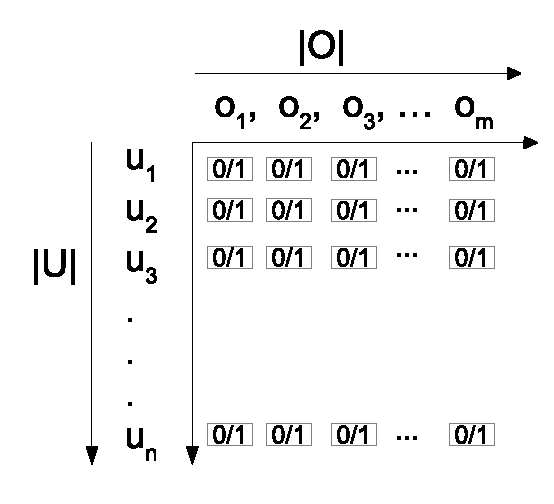
\includegraphics[width=.4\textwidth]{policyspace-hru}
		\caption{LaBAC with one object label and one user label}
		\label{fig:policyspace-hru}
	\end{figure}
 	\begin{figure} 
 		\centering
 		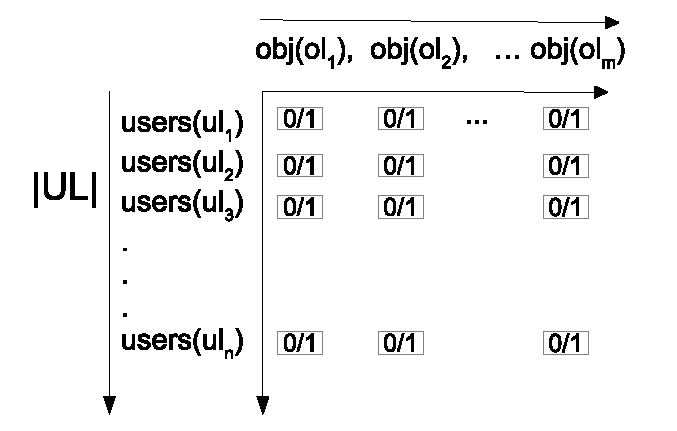
\includegraphics[width=.4\textwidth]{policyspace-labac1}
 		\caption{LaBAC with one object label and one user label}
 		\label{fig:policyspace-labac1}
 	\end{figure}
 	\begin{figure} 
 		\centering
 		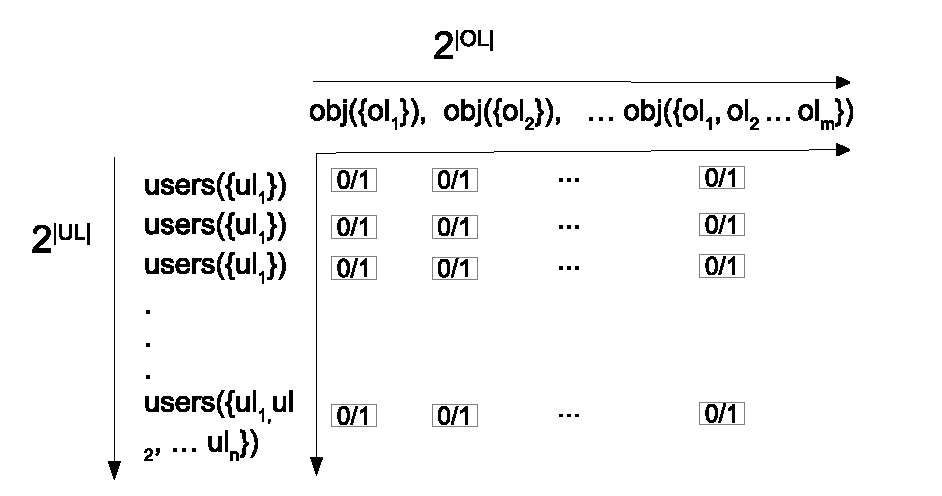
\includegraphics[width=.4\textwidth]{policyspace-labace}
 		\caption{LaBAC with one object label and one user label}
 		\label{fig:policyspace-labace}
 	\end{figure}
% Please add the following required packages to your document preamble:
 % \usepackage{booktabs}
 \begin{table}
 	\centering
 	\caption{Comparison of \policySpace{}}
 	\label{tab:policyspace-comparison}
 	\begin{tabular}{|l|l|}
 		 \hline
 		\textit{HRU \cite{hru}} & $ 2 ^{|U| \times |O|}$ \\
 		\textit{\labacOneOneOne{} } & $ 2 ^{|UL| \times |OL|}$ \\
 		\textit{\elabac} & $ 2 ^{2^{|UL|} \times 2^{|OL|}}$ \\
 		\textit{$\abacAlpha{} \cite{abacAlpha}$} & $2 ^{32}$ \\
 		\textit{\hgabac{}* \cite{hgabac}} & $ 2 ^{2^{|ua_1|} \times 2^{|oa_1|}}$ \\
\hline
 	\end{tabular}
 \end{table} 

 
						
 
%\section{Extensions of LaBAC Model}


\subsection{Extended Policy Model (\elabac)}
% Please add the following required packages to your document preamble:
% \usepackage{booktabs}
\begin{table}
	\centering
	\caption{ \elabac{} Model} %\vspace*{3pt}
	\label{tab:labac-definition}
	\begin{tabular}{|l|}						
		\hline					
		\multicolumn{1}{|c|}{\underline{\textit{I'. New/updated components of the extended model } } }\\	
		- $NUL$ and $NOL$ (set of negated user-labels and \\ \hfill negated object-labels).  $NUL = \{ \lnot ul | \exists ul \in UL\}$ and \\ \hfill  $NOL = \{ \lnot  ol | \exists ol \in OL \}$ \\
		%- $EUL$ and $EOL$ (extended set of user-labels and object-labels). \\ \hfill $EUL = UL \cup NUL$ and  $EOL = OL \cup NOL$ \\
		%- $uLabel$ and $oLabel$ are label functions on users and objects respectively. \\ \hfil Formally, $\uLabel(u:U) \to 2^{\UL}$ and $\oLabel(o:O) \to 2^{\OL}$ \\
		-  $\policy \subseteq 2^{UL \cup NUL} \times A \times 2^{OL\cup NOL}$. \\
		- An individual policy,  $p \in \policy$  \\ \hfil is enumeration of tuples of the form \\ \hfill  $( UL_s \subseteq  UL \cup NUL, a \in \A, OL_s \subseteq OL \cup NOL)$. \\
		%- $\sessionLabels(s:S) \to 2^{UL}$, mapping function from a session to the set of user-labels.  \\ \hfil Formally, 
		%$\sessionLabels(s) \subseteq \{ul' | ul \in uLabel(user(s)) \land ul  \udominate ul'  \}$.		\\ \\
		
	 		  
		
		\multicolumn{1}{|c|}{\underline{\textit{IV. Derived components}}} \\
		- $\impliedPolicy = \{ (UL_t, a, OL_t) | ( \exists (UL_s, a, OL_s) \in \policy) \land$  \\ \hfill $UL_t=\{ ul_j | ( ul_i \in UL_s \cap UL \land ul_j \udominate ul_i) \lor ul_j \in UL_s \cap NUL \} \land$ \\ \hfill $  OL_t=\{ ol_j | (ol_i \in OL_s \cap OL \land ol_i \udominate ol_j\}) \lor ol_i \in OL_s \cap NOL \}$		\\		
	 
		\multicolumn{1}{|c|}{\underline{\textit{V. Authorization functions}}} \\
		- \request(s:S,\amem:A,\objmem:O) =	\\ \hfill  $\exists (UL_s, a, OL_s) \in \policy \cup \impliedPolicy ] \land $   \\
		 \hfill   $\exists ul_i \in UL_s \cap UL \implies  ul_i \in \uLabel(u) \land$ \\
		 \hfill $\exists  ul_i \in UL_s \cap NUL \implies  ul_i \notin \uLabel(u)$ \\
		 \hfill   $\exists ol_i \in OL_s \cap OL \implies  ol_i \in \oLabel(o) \land$ \\
		 \hfill $\exists  ol_i \in OL_s \cap NOL \implies  ol_i \notin \oLabel(o)$ \\

		\\ \hline	
	\end{tabular}
	
\end{table}

%mod



 	\begin{figure}
 		\centering
 		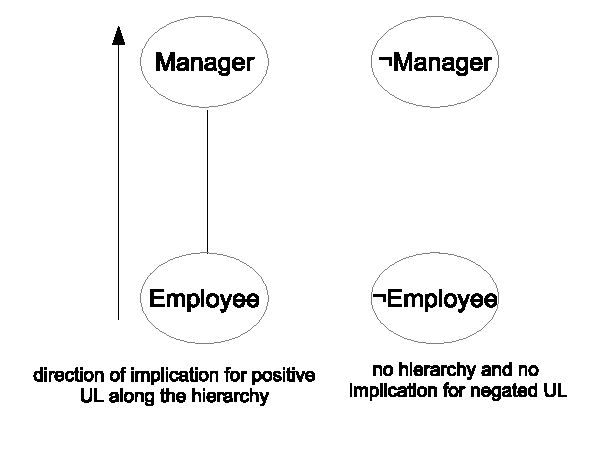
\includegraphics[width=.4\textwidth]{ul-implication}
 		\caption{Implication on UL}
 		\label{fig:ul-implication}
 	\end{figure}

 	\begin{figure} 
 		\centering
 		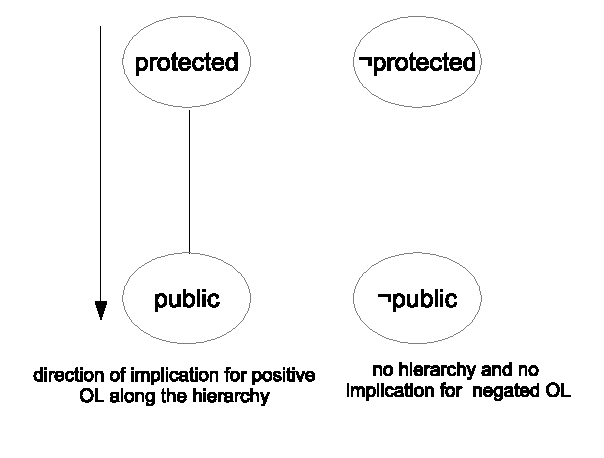
\includegraphics[width=.4\textwidth]{ol-implication}
 		\caption{OL Implication}
 		\label{fig:ol-implication}
 	\end{figure}

\subsection{Multi-label Extensions}
\newcommand{\OLOne}{OL_1}
\newcommand{\OLTwo}{OL_2}
\newcommand{\ULOne}{UL_1}
\newcommand{\ULTwo}{UL_2}
	\begin{figure*} 
		\centering
		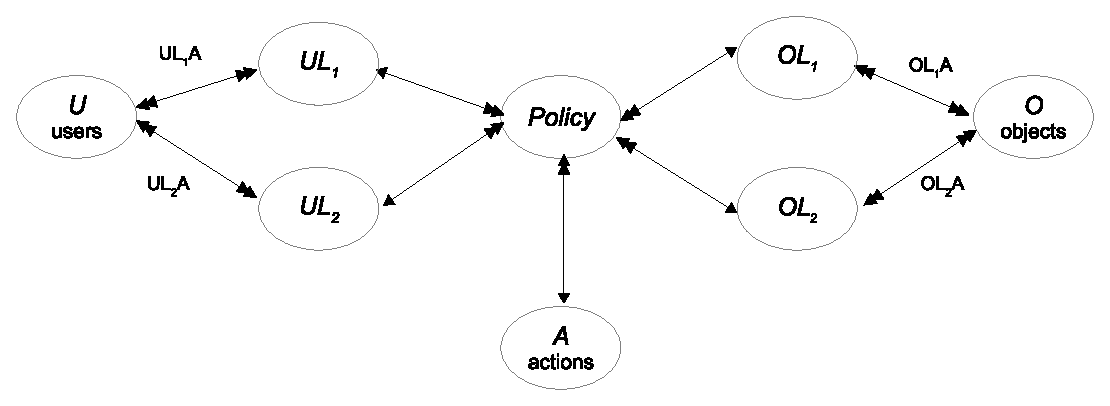
\includegraphics[width=.9\textwidth]{labac22}
		\caption{LaBAC with two object labels and two user labels}
		\label{fig:labac22}
	\end{figure*}

% Please add the following required packages to your document preamble:
% \usepackage{booktabs}
\begin{table}
	\centering
	\caption{ \labacZeroTwoTwo{} Model} %\vspace*{3pt}
	\label{tab:labac022-definition}
	\begin{tabular}{|l|}						
		\hline					
		\multicolumn{1}{|c|}{\underline{\textit{I. Component of the basic model }}}\\			
		- $U, O$, $A$ and $S$ (set of users, objects, actions and \\ \hfill sessions respectively).  \\
		- $\ULOne, \ULTwo, \OLOne, \OLTwo$ (set of $uLabel_1, uLabel_2,$ \\ \hfill $oLabel_1$ and $oLabel_2$ values respectively). \\
		- $\uLabelOne, \uLabelTwo, \oLabelOne, \oLabelTwo$ are label functions \\ \hfill on users and objects respectively. Formally, \\ \hfill  $\uLabelOne(u:U) \to 2^{\ULOne}$ and $\oLabelOne(o:O) \to 2^{\OL1}$ \\ \hfill  $\uLabelTwo(u:U) \to 2^{\ULTwo}$ and $\oLabelTwo(o:O) \to 2^{\OL2}$ \\  
		-  $\policy_a \subseteq \ULV_1 \times \ULV_2 \times \OLV_1 \times \OLV_2$ \\
		 %An individual policy,   $p \in \policy$  is \\ \hfil enumeration of tuples of the form $( ul_1 \in UL_1, ul_2 \in UL_2, a \in \A, ol_1 \in OL_1, ol_2 \in OL_2)$. \\
	 
		 - $\sessionLabels(s:S) \to 2^{UL_1 \times UL_2}$, mapping function from \\ \hfill a session   to the set  of $\uLabelOne{}$ and $\uLabelTwo{}$ values.    \\ \hfill formally	$\sessionLabels(s) \subseteq \{(ul_1', ul_2') | ul_1 \in \uLabelOne(user(s)) \land$ \\ \hfill $ul_1  \udominate ul_1' \land$   $ul_2 \in \uLabelTwo(user(s)) \land ul_2  \udominate ul_2' \}$.		\\ \\
		
		\multicolumn{1}{|c|}{\underline{\textit{V. Authorization functions}}} \\
		- \request(u:U,\amem:A,\objmem:O) =	 \\ \hfill
		$\exists ul_1 \in \uLabelOne(u) \land ul_2 \in \uLabelTwo(2) \land$ $ ol_1 \in \oLabelOne(o) \land$ \\ \hfill  $ ol_2 \in \oLabelTwo(o) \land  (ul_1, ul_2,ol_1, ol_2) \in \policy_a   $  

		\\ \hline	
	\end{tabular}
	
\end{table}

%mod



	\begin{figure} 
		\centering
		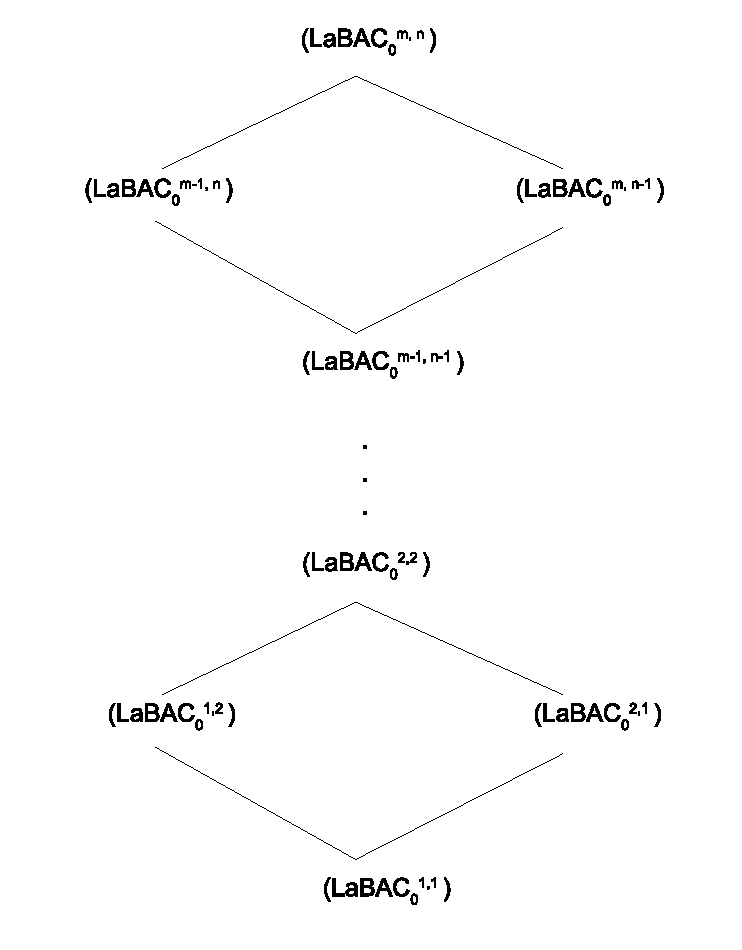
\includegraphics[width=.4\textwidth]{labacmn-family}
		\caption{LaBAC family of model extended with m object labels and n user labels.}
		\label{fig:labacmn-family}
	\end{figure}

\subsection{Expressive power of  \labacZeroOneOne vs \labacZeroMN}

% Please add the following required packages to your document preamble:
% \usepackage{booktabs}

\begin{table}
	\centering
	\caption{  \labacZeroTwoTwo{} in \labacZeroOneOne{}} %\vspace*{3pt}
	\label{tab:lbac-in-labac}
	\begin{tabular}{|l|}						
		\hline					
		\multicolumn{1}{|c|}{\underline{\textit{I. \labacZeroTwoTwo{} Components }}}\\	
		 - $U^{2,2}, O^{2,2}, A^{2,2}$	\\		 
	     - $UL_1, UL_2, OL_1, OL_2$\\
		 -  $\uLabelOne(), \uLabelTwo(), \oLabelOne(), \oLabelTwo()$ \\
		 -  $\policy^{2,2}_a \subseteq  UL_1 \times UL_2 \times OL_1 \times OL_2$\\	 
		\multicolumn{1}{|c|}{\underline{\textit{III. Construction}}} \\
		 - $U = U^{2,2}, O = O^{2,2}, A = A^{2,2}$\\
		 -  $UL = UL_1 \times UL_2$ \\
		 - $OL = OL_1 \times OL_2$\\		 
		 -  $  \uLabel(u) =  \uLabelOne(u) \cup \uLabelTwo(u)$ \\
		 -  $  \oLabel(o) =  \oLabelOne(o) \cup \oLabelTwo(o)$ \\ 
		 - $ \policy_{a} = \{ ( (UL_1 \times UL_2) \times (OL_1 \times OL_2))|$ \\ \hfill $(ul1, ul2, ol1, ol2) \in \policy_a \}$ \\
		 - Def. of  $\sessionLabels(s)$ for session $s \in S$  and \\ \hfill $\request(s, a, o)$   are unchanged 	\\	
	 
		\\ \hline	
	\end{tabular}	
\end{table}

%\section{Discussion on ABAC Policy}
%


\subsection { Implementation in OpenStack Swift}
\label{sec:implementation}

 \begin{figure} [t]
 	\centering
 	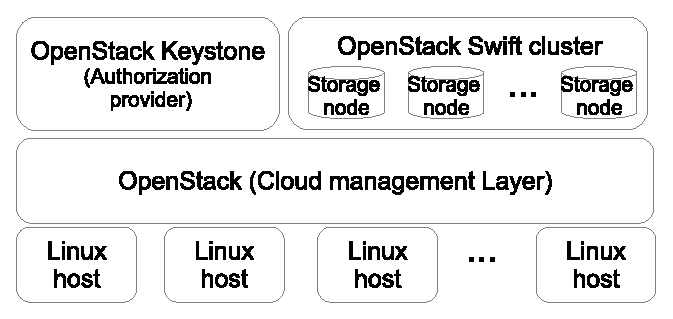
\includegraphics[width=.6\textwidth]{NSS16/reference-implementation-architecture}
 	\caption{Reference architecture of the implementation testbed}
 	\label{fig:reference-implementation-architecture}
 \end{figure}


 
 	\begin{figure} [t]
 		\centering
 		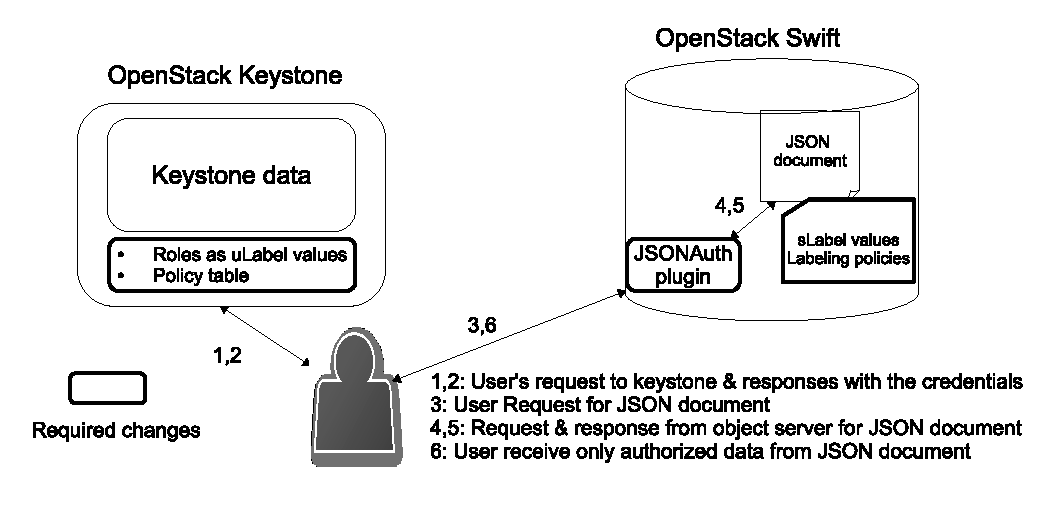
\includegraphics[width=.9\textwidth]{NSS16/implementation-in-swift}
 		\caption{Implementation in OpenStack IaaS cloud platform}
 		\label{fig:implementation-in-swift}
 	\end{figure}
 

We have implemented our proposed operational model and path-based labeling scheme in OpenStack IaaS cloud platform using OpenStack Keystone as the authorization service provider and OpenStack Swift as the storage service provider. Our choice of OpenStack is motivated by its support for independent and inter-operable  services and a well defined RESTful API set.

We have modified OpenStack Keystone and Swift services to accommodate required changes. A reference architecture of our testbed is given in Figure \ref{fig:reference-implementation-architecture}. Details of the implementation is shown in Figure \ref{fig:implementation-in-swift-a}. Required changes are presented as highlighted rectangles in Figure \ref{fig:implementation-in-swift-a}.

\subsection{Changes in OpenStack Keystone}

 OpenStack Keystone uses roles and role-based policies to provide authorization decisions. In our implementation, we uses roles to hold user-label attribute values. A set of valid security-label values are also stored as part of the Keystone service.
 
 Among two different types of policies, authorization and labeling policies, the former is managed in the Keystone service. We assume, a higher level administrators (possibly at the level of organization) adds, removes or updates these authorization policies. We add a policy table in Keystone database to store these enumerated authorization policies. 

\subsection{Changes in OpenStack Swift}

In Swift side, we store \textit{security-label} values assigned to JSON objects and path-based labeling policies applied to them.  Security-label values and labeling policies are stored as metadata of the stored objects, which are JSON documents in this case. For simplicity, we assume object owner (Swift account holder in this case) can update security-label values or labeling policies for a stored JSON document. 


 During the evaluation, we intercept every request to Swift (from the Swift-proxy server) and reroute the request to be passed through \textit{JSONAuth plugin}, if it is a request for a JSON document. In this case, the request additionally carries a requested path and authorization policies applicable to the user. JSONAuth plug-in retrieves the requested JSON document, applies path-based labeling policies to annotate the document and uses authorization policies to determine if the user is authorized for the requested content of the file. 

\subsection{Evaluation}

 \begin{figure} [t]
 	\centering
 	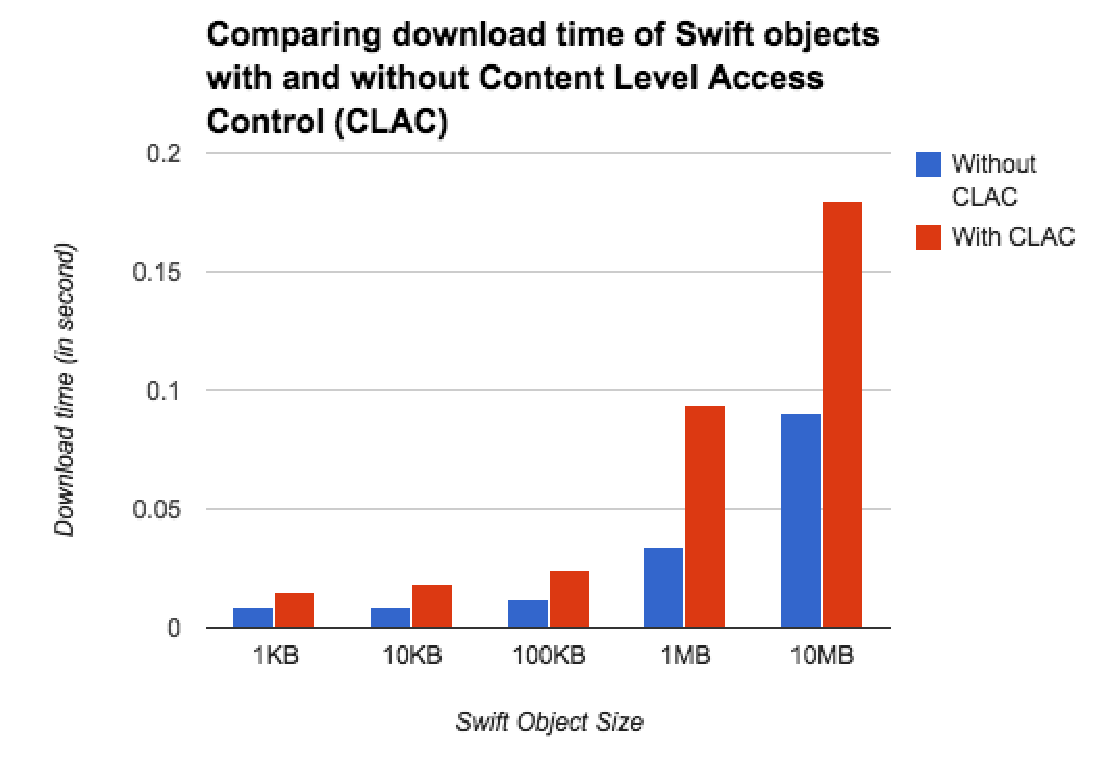
\includegraphics[width=.9\textwidth]{NSS16/performance}
 	\caption{Performance evaluation}
 	\label{fig:performance-a}
 \end{figure}


An evaluation of our implementation is shown in Figure \ref{fig:performance-a}. The evaluation has been made against concurrent download requests to the Swift proxy server. The X-axis shows size of the JSON document requested for download while the Y-axis shows the average download time for 10 concurrent request. Our evaluation shows a performance hit of nearly 60\% over no authorization protection.
%\textbf{Performance}



\section{Conclusion \& Future work}
\label{sec:conclusion}


In this paper, we present a simple Attribute Based Access Control model (LaBAC) using enumerated policies. LaBAC is based on single user attribute ($\uLabel$) and single object attribute ($\oLabel$). We analyze LaBAC with other enumerated policy models. LaBAC can be viewed as a simple instance of an existing enumerated policy model - Policy Machine. LaBAC is also equivalent to \twoSortedRBAC{}, which is the other enumerated policy model as we are aware of. We show flexibility of LaBAC in terms of configuring traditional models (RBAC and LBAC) in it. 

Besides enumerated policy, we also discuss logical formula based authorization policy which is the more conventional approach for designing ABAC policy.  Logical formula can be very rich and complex and capable of expressing even complicated business logic in a very succinct form. But policy review or policy update may become NP-complete in policies expressed in logical formulas. 
%We believe, reviewing or updating policy would be  crucial in maintaining an ABAC system. This motivates us to explore other avenues in the design of an ABAC model. 

Enumerated policies as an alternate to specify authorization policies raise many interesting issues that need to be addressed to better  understand the nature of ABAC. For example, are there other alternates to specify authorization policies or policies in general in a ABAC system? What are the pros and cons of using logical formula or enumerated policy? Does review of policy or policy update become any simple in enumerated policies?  

Additionally, many other questions need to be addressed in term of enumerated policy ABAC models. Are enumerated policy models as expressive (or less/more) as logical formula based models? How (if possible) can we express arbitrary business logic in enumerated policies? What would be the cost of storing potentially large number of enumerated tuples? How can we extend LaBAC to incorporate more than one user and object labels (or attributes) and so on?

%On the contrary, enumerated policy is simple and policy review in it is inherently polynomial time. But there are many issues we need to be addressed in term of enumerated policy model. Is enumerated policy model less (or equal/more) expressive in general than logical formula based model?  Is there a  trade-off between expressive power and complexity of policy review/policy update? What would be the cost of storing potentially large number of enumerated polices? Are there alternates of designing ABAC policy other than or in between two extremes of logical formula and enumerated tuples and so on. 
\begin{acknowledgements}
First of all, I would like to thank Kevin Xu Su for creating an earlier
version of the \LaTeX{} style, Lijie Zhang for using an earlier version
of this package to write her dissertation and to provide feedback. 

I would also like to thank the UTSA Graduate School for reviewing
the outcome of this template document and correction of formatting
errors. 

(Notice: If any part of the thesis/dissertation has been published
before, the following two paragraphs should be included without alteration).

\begin{singlespace}
\emph{This Masters Thesis/Recital Document or Doctoral Dissertation
was produced in accordance with guidelines which permit the inclusion
as part of the Masters Thesis/Recital Document or Doctoral Dissertation
the text of an original paper, or papers, submitted for publication.
The Masters Thesis/Recital Document or Doctoral Dissertation must
still conform to all other requirements explained in the Guide for
the Preparation of a Masters Thesis/Recital Document or Doctoral Dissertation
at The University of Texas at San Antonio. It must include a comprehensive
abstract, a full introduction and literature review, and a final overall
conclusion. Additional material (procedural and design data as well
as descriptions of equipment) must be provided in sufficient detail
to allow a clear and precise judgment to be made of the importance
and originality of the research reported. }

\emph{It is acceptable for this Masters Thesis/Recital Document or
Doctoral Dissertation to include as chapters authentic copies of papers
already published, provided these meet type size, margin, and legibility
requirements. In such cases, connecting texts, which provide logical
bridges between different manuscripts, are mandatory. Where the student
is not the sole author of a manuscript, the student is required to
make an explicit statement in the introductory material to that manuscript
describing the students contribution to the work and acknowledging
the contribution of the other author(s). The signatures of the Supervising
Committee which precede all other material in the Masters Thesis/Recital
Document or Doctoral Dissertation attest to the accuracy of this statement.}\end{singlespace}
\end{acknowledgements}

\bibliographystyle{abbrv}
\bibliography{sigproc}
%\clearpage
%%\textbf{Appendix}
\section{Appendix}
\vspace{-1.5em}
%\vspace{-1em}
\renewcommand{\suffix}{m,n}
\newcommand{\suffixT}{1,1}
\begin{table}
	\centering
	\caption{ Mappings } %\vspace*{3pt}
	\label{tab:lp11-to-lpmn}
	\begin{tabular}{|l|}						
		\hline					
%			\multicolumn{1}{|c|}{\underline{\textit{I. \LPOneOne{} components}}} \\
%				  - $U, O, A, S, UAV, OAV$  (users,  objects, actions, subjects, user and object attr. values.)\\
%				  - $ua,oa$ (attribute functions);  $ua:U\to 2^{UAV}$; $oa:O\to 2^{OAV}$ \\ 
%				  - $\subCreator: S \to U$ ; $sa:S\to 2^{UAV}$,    $sa(s) \subseteq ua(\subCreator(s))$\\
%				  - $f_a: (sa(u), oa(o)) \to \{true, false\}$  and $\isAuthorized(s,a,o) =(f_a(sa(u),oa(o))=true$) \\
				 
		   
		   \multicolumn{1}{|c|}{\underline{\textit{I. From \LPMN{} to \LPOneOne{}}}}\\	
			   - $U = U_{\suffix}; O = O_{\suffix}; A = A_{\suffix}; S = S_{\suffix};$$\textit{UAV} = \UAV{1} \times \UAV{2}\times ... \times \UAV{m}$\\
			   -  $\textit{OAV} = \OAV{1} \times \OAV{2}\times ... \times \OAV{m}$;$ua(u) = \ua{1}(u) \times \ua{2}(u) \times ... \times \ua{m}(u) $\\
			   -$oa(u) = \oa{1}(u) \times  ... \times \oa{m}(u) $$sa(u) = \sa{1}(u) \times ... \times \sa{m}(u) $; $\creator(s) = \creator_{\suffix}(s)$\\
			    - $ f_a =$ $\mathop{\bigvee}\limits_{ f_{a_{m,n}}( \ULS{1}, \ULS{2},...\ULS{m}, \OLS{1}, \OLS{2}, ...,\OLS{n})=true }  (\ULS{1}(u) \times ... \times \ULS{m}(u) \subseteq ua(u) )\land$ \\ \hfill  $(\OLS{1}(o) \times ... \times \OLS{n}(o) \subseteq oa(o))$, for $\ULS{i} \subseteq \UAV{i}$ and $\OLS{i} \subseteq \OAV{i}$ \\ 		
			   
 
	   \multicolumn{1}{|c|}{\underline{\textit{II. From \LPOneOne{} to \LPMN{}}}}\\	
			- $U = U_{\suffixT}; O = O_{\suffixT}; A = A_{\suffixT}; S = S_{\suffixT};$\\
			- $\UAV{1} = UAV; \UAV{2} = \{\}; ... \UAV{m} = \{\};$  $\OAV{1} = OAV; \OAV{2} = \{\}; ... \OAV{n} = \{\};$\\
			- $\ua{1}(u) = ua(u); \ua{2}(u) = \{\};...\ua{m}(u) = \{\}$; $\oa{1}(o) = oa(o); \oa{2}(o) = \{\};...\oa{m}(o) = \{\}$\\
		    - $\sa{1}(u) = sa(u); \sa{2}(u) = \{\};...\sa{m}(u) = \{\}$; $\creator_{\suffix}(s) = \creator(s)$ and $f_{a_{\suffix}} =$\\
		    $\mathop{\bigvee}\limits_{ f_{a}( \ULS{i},\OLS{i})=true }  (\ULS{i} \subseteq \ua{1}(u) \land$   $ \OLS{i}\subseteq oa(o))$  for $\ULS{i} \subseteq UAV$ and $\OLS{i} \subseteq OAV$ \\ 
		 %\hline	
		 	\multicolumn{1}{|c|}{\underline{\textit{III. From \EPOneOneModels{} to \LPOneOne{} }}}\\					
		 	- $U  = U ; O  = O ; A  = A $; $UAV	= UL; OAV = OL$;$ua(u) = uLabel(u)$; $oa(o)=oLabel(o) $\\
		 	-  $sa(s) = \sessionLabels(s) $ ;$f_a =$ $\mathop{\vee}\limits_{ (ul_i, ol_i) \in \policy_a} ( ul_i \in ua(u) \land ol_i \in oa(o))$. \\
		 	
		 	\multicolumn{1}{|c|}{\underline{\textit{IV. From \LPOneOne{} to \EPOneOneModels{}}}}\\	
		 	- $UL= 2^{ULV}; OL= 2^{OLV}; \uLabel(u) = 2^{ua(u)};\oLabel(o) = 2^{oa(o)}; \sessionLabels(s) = 2^{sa(s)}$ \\	  
		 	- $\Policy_a = \{  (\ulsubset, \olsubset) | (\exists \ulsubset \subseteq UL, \exists \olsubset \subseteq OL)[ f_a(\ulsubset, o\ulsubset) = true] \} $
		 	
		 	\\ \hline	
	\end{tabular}	

	
\end{table}
%\vspace{-1.5em}
\vspace{-1.5em}
\subsubsection{Tripli equivalence}
\EPOneOneModels{}  $\equiv $($\myGamma{1,1}, \myQ{1,1}, \myvdash{1,1}, \myPSI{1,1}$) where a state,  $ \mygamma{}{1,1} \in \myGamma{1,1}$ is  $(U, O, A, S, uLabel, oLabel,$ $ \sessionLabels{},  UL,$  $ OL, \Policy)$. $\myPSI{1,1} =  \{\createSession,$ $ \assignValues,$ $ \removeValues, \deleteSession\}$. $\myQ{1,1}=\{ \myq{s}{1,1} \equiv \isAuthorized(s, a, o)|$  $ a\in A, s \in S, o \in O \}$. $\mygamma{}{1,1} \myvdash{1,1} \myq{s}{1,1}$ iff $\isAuthorized(s,a,o)$ $=true$. 

\EPMNModel{} $\equiv$ ($\myGamma{m,n}, \myQ{m,n}, \myvdash{m,n},\myPSI{m,n}$ ) where  $ \mygamma{}{m,n} \in \myGamma{m,n}$ is  $(U, O, A, S, \uLabelP{1},..\uLabelP{m}, \oLabelP{1},..\oLabel{n},$ $ \sessionLabelsP{1},..\sessionLabelsP{m},  \UL{1},..\UL{m},$  $ \OL{1},..\OL{n}, \Policy)$. $\myPSI{m,n} =  \{\createSession,$ $ \assignValues,$ $ \removeValues, \deleteSession\}$. $\myQ{m,n}=\{ \myq{s}{m,n} \equiv \isAuthorized$ $(s, a, o) \}$. $\mygamma{}{m,n} \myvdash{m,n} \myq{s}{m,n}$ iff $\isAuthorized(s,a,o)$ $=true$.

let $\mygamma{0}{1,1}$ and $\mygamma{0}{m,n}$ be the start state of \EPOneOneModels{} and \EPMNModel{} using mapping in Segment III of Table \ref{tab:mapping-epmn-ep11}. let $\mygamma{0}{1,1} \myvdash{1,1} \myq{s}{1,1}$. i.e. $ \isAuthorized(u,a,o) = true \land (ul,ol) \in \Policy_a$ and $ul \in uLabel(u) \land ol \in oLabel(o)$ in $\mygamma{0}{1,1}$. According to mapping, $(\{ul\},\{\}... \{ol\}.. \{\}) \in \Policy_a$ in $\mygamma{0}{m,n}$. Thus, $\mygamma{0}{m,n} \myvdash{m,n} \myq{0}{m,n}$. So, the initial states are equivalent. Now, for each state transition in $\myPSI{1,1}$ there exists a transition in $\myPSI{m,n}$. For example, $\createSession$ exists in both $\myPSI{1,1}$ and $\myPSI{m,n}$. We can use the same logic of initial states so show that every reachable states using the transition is also equivalent. This proves the current mapping is a state matching reduction. Similarly, we can show the same result for the other mapping. Thus \EPOneOneModels{} and \EPMNModel{} are equivalent.

\vspace{-1em}
%% Please add the following required packages to your document preamble:
% \usepackage{booktabs}
\begin{table}
	\centering
	\caption{ Mapping from \EPOneOneModels{} to \LPOneOne{} and vice versa } %\vspace*{3pt}
	\label{tab:lp11-to-ep11}
		\begin{tabular}{|l|}						
		\hline		
	\multicolumn{1}{|c|}{\underline{\textit{I. From \EPOneOneModels{} to \LPOneOne{} }}}\\					
	- $U  = U ; O  = O ; A  = A $; $UAV	= UL; OAV = OL$;$ua(u) = uLabel(u)$; $oa(o)=oLabel(o) $\\
	-  $sa(s) = \sessionLabels(s) $ ;$f_a =$ $\mathop{\vee}\limits_{ (ul_i, ol_i) \in \policy_a} ( ul_i \in ua(u) \land ol_i \in oa(o))$. \\
	 
	 \multicolumn{1}{|c|}{\underline{\textit{II. From \LPOneOne{} to \EPOneOneModels{}}}}\\	
	  - $UL= 2^{ULV}; OL= 2^{OLV}; \uLabel(u) = 2^{ua(u)};\oLabel(o) = 2^{oa(o)}; \sessionLabels(s) = 2^{sa(s)}$ \\	  
	 - $\Policy_a = \{  (\ulsubset, \olsubset) | (\exists \ulsubset \subseteq UL, \exists \olsubset \subseteq OL)[ f_a(\ulsubset, o\ulsubset) = true] \} $

		 \\ \hline	
	\end{tabular}
	
\end{table}

%mod





%


%\subsection{Functional Specification}
\label{sec:session-management}
\begin{table*}
\centering
\caption{User-level session functions in \clabac{}}
\label{tab:session-management}
\begin{tabular}{|l|l|l|}
	\hline
\textbf{Fuction}                                                              & \textbf{Condition} & \textbf{Updates} \\ \hline

%\begin{tabular}[c]{@{}l@{}}\createSession\\ (u:U, s:S, values)\end{tabular} & \begin{tabular}[c]{@{}l@{}} $u \in U \land s \not \in S \land values \subseteq \uLabel(u) \setminus \{\createReq, \removeReq\}\  $ \\ $\createReq \in \uLabel(u) \land $ \\ $\exists\Policy_{\createSession} \equiv \{(\createReq, \sessionOL) \}\in \Policy$ \\ \end{tabular} &  \begin{tabular}[c]{@{}l@{}}$S' = S \cup \{s\}$ \\ $\creator(s) = u \land \sessionLabels(s)=value $ \end{tabular} \\\hline
%\multicolumn{3}{c}{\textbf{\textit{User level functions}}}\\ \hline

\begin{tabular}[c]{@{}l@{}}$\createSession$\\ $(u:U, s:S, values:2^{UL}$)\end{tabular} & \begin{tabular}[c]{@{}l@{}} $u \in U \land s \not \in S \land values \subseteq \uLabel(u)$  \end{tabular} &  \begin{tabular}[c]{@{}l@{}}$S' = S \cup \{s\}$,  $\creator(s) = u ,$ \\ $ \sessionLabels(s)=value $ \end{tabular} \\\hline


\begin{tabular}[c]{@{}l@{}}$\deleteSession$\\ $(u:U, s:S)$\end{tabular}   & \begin{tabular}[c]{@{}l@{}} $u \in U \land s  \in S \land creator(s)=u  $ \end{tabular}                   & \begin{tabular}[c]{@{}l@{}}$S' = S \setminus \{s\}$ \end{tabular}                             \\\hline


\begin{tabular}[c]{@{}l@{}}$\assignValues$\\ $(u:U,s:S, values:2^{UL}$)\end{tabular} &  \begin{tabular}[c]{@{}l@{}} $u \in U \land s  \in S \land creator(s)=u \land  values \subseteq \uLabel(u)$ \end{tabular} &   \begin{tabular}[c]{@{}l@{}} $\sessionLabels(s)= \sessionLabels(s) \cup values $ \end{tabular}                \\ \hline


\begin{tabular}[c]{@{}l@{}}$\removeValues$\\ $(u:U,s:S, values:2^{UL}$)\end{tabular} &  \begin{tabular}[c]{@{}l@{}} $u \in U \land s  \in S \land creator(s)=u \land   values \subseteq \uLabel(u)$ \end{tabular} &   \begin{tabular}[c]{@{}l@{}} $\sessionLabels(s)= \sessionLabels(s) \setminus values $ \end{tabular}                \\ \hline

%\begin{tabular}[c]{@{}l@{}}$\createObject$\\ $(s:S, o:O, values:2^{OL}$)\end{tabular} &  \begin{tabular}[c]{@{}l@{}} $s \in S \land o \not \in O \land $ \\$ f_{\createObject}(s,o, values) $ \end{tabular} &   \begin{tabular}[c]{@{}l@{}} $O' = O \cup \{o\}, \oLabel(o) = values$ \end{tabular}                \\ \hline

%\begin{tabular}[c]{@{}l@{}}$\assignLabels$\\ $(s:S, o:O, values:2^{OL}$)\end{tabular} &  \begin{tabular}[c]{@{}l@{}} $s \in S \land o  \in O \land $ \\$ f_{\assignLabels}(s,o, values) $ \end{tabular} &   \begin{tabular}[c]{@{}l@{}} $ \oLabel(o) = \oLabel(o) \cup values  $ \end{tabular}                \\ \hline

%\begin{tabular}[c]{@{}l@{}}$\removeLabels$\\ $(s:S, o:O, values:2^{OL}$)\end{tabular} &  \begin{tabular}[c]{@{}l@{}} $s \in S \land o  \in O \land $ \\$ f_{\removeLabels}(s,o, values) $ \end{tabular} &   \begin{tabular}[c]{@{}l@{}} $ \oLabel(o) = \oLabel(o) \setminus values  $ \end{tabular}                \\ \hline


%\begin{tabular}[c]{@{}l@{}}\removeValues\\ (u:U,s:S, values:2)\end{tabular} &  \begin{tabular}[c]{@{}l@{}} $u \in U \land s  \in S \land $  $\creator(s) = u \land $ $ \removeReq \in \uLabel(u) $ \\ \end{tabular} &   \begin{tabular}[c]{@{}l@{}} $\sessionLabels(s)= \sessionLabels(s) \setminus values $ \end{tabular}                \\ \hline
                 
\end{tabular}
\end{table*}



\eapABAC{} allows users to create or destroy sessions, and assign/remove values from an existing session. Table \ref{tab:session-management} presents user-level \textit{\sessionLabels{}} functions for managing sessions in \clabac{}. Each function is presented with formal parameters (given in the first column), necessary preconditions (in the second column) and resulting updates (in the third column).  The function $\createSession()$ creates a new session with given values, $\deleteSession()$ deletes an existing session, $\assignValues()$ assigns values in an existing session, and $\removeValues()$ removes values from an existing session. 

%First column in the table shows function names along with formal parameters, second column defines precondition which must be satisfied for the function to be executed. The third column describes updates in the LaBAC sets and relations once corresponding function is executed.

In \hlabac{}, we modify condition of the session functions from Table \ref{tab:session-management} to accommodate  that in a session created by a user, he can choose from the values he is assigned to or junior values. The modified conditions are given in Table \ref{tab:session-in-hlabac}. We specify an additional condition with each session function  in \consLabac{} and \labacOneOneOne{}.  For example, with $\createSession()$,  we specify a boolean function $f_{\createSession}()$ as additional precondition which must also be true. The definition of these boolean functions are  open-ended to be able to configure any session constraints. The difference between session functions in \consLabac{} and \labacOneOneOne{} is that the former does not consider hierarchy on user-label values whereas the later does. Table \ref{tab:session-in-consLabac} and \ref{tab:session-in-labacOne} show session functions in \consLabac{} and \labacOneOneOne{} respectively. Table \ref{tab:example-f-create-session} presents some examples of constraints specified with $f_{\createSession}()$ function.  \textit{Example 1} uses an enumerated policy, $\Policy_{\createSession}$. It specifies that in order to create a session and assign values to the session, a user must be assigned to value $\createReq$. \textit{Example 2} enforces the constraint that no more than one conflicting $\uLabel$ values can be activated in a session. \textit{Example 3} imposes that a user cannot have more than some bounded number of sessions.

Note that creation and deletion of objects, updating object-label values by sessions are outside the scope of \eapABAC{} operational models presented here. One reason behind is that, \eapABAC{} only focuses on attributes. It can be extended to include object creation and modification along the line of $ABAC_{\alpha}$ \cite{abacAlpha}. See Table \ref{tab:lbac-in-labac} for example.

\begin{table} 
\centering
 \captionsetup{justification=centering}
\caption{Session functions in \hlabac{} \newline (condition of session functions modified from Table \ref{tab:session-management} ) }
\label{tab:session-in-hlabac}
\begin{tabular}{|l|l|} \hline
\textbf{Function} & \textbf{Modified condition} \\ \hline
  $\createSession{}$      & \begin{tabular}[c]{@{}l@{}}  $u \in U \land s \not \in S \land values \subseteq$ \\ \hfill$  \{ ul' | \exists ul \udominate ul' [ ul \in \uLabel(u)] \}$ \end{tabular}             \\ \hline
	$\deleteSession{} $        & $u \in U \land s  \in S \land creator(s)=u  $                     \\ \hline
     $\assignValues{}$    &     \begin{tabular}[c]{@{}l@{}}  $u \in U \land s  \in S \land creator(s)=u \land values $ \\ \hfill$  \subseteq \{ ul' | \exists ul \udominate ul' [ ul \in \uLabel(u)] \}$ \end{tabular}                \\ \hline
 $\removeValues{}$    &     \begin{tabular}[c]{@{}l@{}}  $u \in U \land s  \in S \land creator(s)=u  \land values $ \\ \hfill$  \subseteq \{ ul' | \exists ul \in  \uLabel(u) \land ul \udominate ul' \}$ \end{tabular}                 \\ \hline
\end{tabular}
\end{table}



\begin{table}[]
\centering
 \captionsetup{justification=centering}
\caption{Session functions in  \consLabac{} (condition added with session functions from Table \ref{tab:session-management})}
\label{tab:session-in-consLabac}
\begin{tabular}{|l|l|} \hline
\textbf{Session function} & \textbf{Additional condition} \\ \hline
   $\createSession{}$      & $\land f_{\createSession}(u,s,values)$               \\ \hline
	$\deleteSession{} $        & $\land f_{\deleteSession}(u,s)$                     \\ \hline
     $\assignValues{}$    &      $\land f_{\assignValues}(u,s,values)$                \\ \hline
 $\removeValues{}$    &      $\land f_{\removeValues}(u,s,values)$                \\ \hline
\end{tabular}
\end{table}

\begin{table}[]
\centering
 \captionsetup{justification=centering}
\caption{Session functions in  \labacOneOneOne{} (condition added with session functions from Table \ref{tab:session-in-hlabac})}
\label{tab:session-in-labacOne}
\begin{tabular}{|l|l|} \hline
\textbf{Session function} & \textbf{Additional condition} \\ \hline
   $\createSession{}$      & $\land f_{\createSession}(u,s,values)$               \\ \hline
	$\deleteSession{} $        & $\land f_{\deleteSession}(u,s)$                     \\ \hline
     $\assignValues{}$    &      $\land f_{\assignValues}(u,s,values)$                \\ \hline
 $\removeValues{}$    &      $\land f_{\removeValues}(u,s,values)$                \\ \hline
\end{tabular}
\end{table}



\begin{table}
	\centering
 \caption{Examples of $f_{\createSession}(u, s, values)$}
 \label{tab:example-f-create-session}
	\begin{tabular}{|l|}
		\hline	                                                                                           	
		%\multicolumn{1}{|c|}{\underline{\textit{Examples in \consLabac{}/\labacOneOneOne{}:}}}\\                	
		\multicolumn{1}{|l|}{{\textit{Example 1. using LaBAC policy:}}}\\
		
		$\exists \createReq \in \uLabel(u) \land$ \\$ \exists \Policy_{\createSession} \equiv \{(\createReq, \sessionOL) \}\in \Policy$ \\
		
		\\ \multicolumn{1}{|l|}{{\textit{Example 2. using \labacOneOneOne{} session constraint CSL:}}}\\
		 $|values \cap OneElement(CSL)| <= 1$ \\
		 
		 \\\multicolumn{1}{|l|}{{\textit{Example 3. using cardinality  constraint on sessions:}}}\\
		 $|\{s | \creator(s)=u\}| <= 10$ \\
		 \hline
		\end{tabular}  

\end{table}


\end{document}
